% ----------------------------------------------------------------------

\newpage

\subsection{\phopt Test}
\label{ss:phoptimization}

\subsubsection{Purpose}

The \phopt test is responsible for setting an appropriate dynamic range for the 8-bit ADC that digitizes the recorded pulse height.
The ADC is located in the Controller and Interface Block of the \roc.
It can be seen in the bottom right box of Figure~\ref{fig:puc}.
The two \dacs used to configure the ADC are \phoffset and \phscale.
\phoffset adds a constant offset to the pulse height measurement,
while \phscale effectively sets the gain of the ADC.
The \phopt test is designed to optimize these \dacs based on a highly sensitive and highly insensitive pixel in the given \roc, 
or, in other words, pixels with a very high and very low inherent gain.
To use the ADC most effectively, the range of the ADC PH response as a function of \vcal needs to be optimized.
On the low end, the ADC should provide a PH well above noise for the low-gain pixel near the lowest \vcal that registers a hit on it.
On the high end, the ADC should saturate for the high-gain pixel at some user-defined \vcal well below the maximum \vcal the \roc can provide.
This allows the signal strength required for saturation to be measured and recorded for all pixels.
These two conditions are translated into two constraints used to simultaneously find a solution for the values of \phoffset and \phscale.
The constraints applied are 1: the low-gain pixel should have a reasonably large PH (default is 20) at its \vcal turn-on threshold,
and 2: the high-gain pixel should saturate (PH reaches 255) at a user-defined signal strength (default is \vcal = 100 (high range)).

\subsubsection{Methodology}

The \phopt test proceeds in two steps:  
First, it identifies a low-gain and high-gain pixel for use in optimizing \phscale and \phoffset.
In this process, care is taken not to choose anomalous pixels.
Secondly, it maps the pulse height responses of these two pixels as a function of \phscale and \phoffset.
The maps for these two pixels are then combined to find the optimal values for \phscale and \phoffset.
After the optimal values for \phscale and \phoffset are set, several validation plots are made and recorded in the output file.
\\\\
First, the test identifies a low-gain and high-gain pixel using the same methodology for each.
Pixels within 3 columns or 5 rows of the edge of the \roc are not considered, 
unless a suitable pixel cannot be found using those fiducial cuts, in which case those requirements are relaxed.
In each case, the PH for each pixel is obtained at a chosen \vcal (Figures~\ref{fig:phopt_minphmap},~\ref{fig:phopt_maxphmap}), 
and a 1D distribution of all PHs is created for each \roc (Figures~\ref{fig:phopt_dist_minphmap},~\ref{fig:phopt_dist_maxphmap}). 
From this distribution, a pixel is chosen that is separated from the edge of the distribution by a chosen percentile of safety margin.
This helps avoid choosing an anomalous pixel.
For finding the high-gain pixel, this process is performed with the maximum calibration pulse strength, \vcal=255 (high range).
The safety margin is configurable, and by default is 98\%, i.e. a pixel will be chosen such that 98\% of pixels in the \roc have lower PHs.
For finding the low-gain pixel, the process is performed with a \vcal slightly higher than the \vcal trimming target, 
hard-coded to \vcal=60 (low range).
For the chosen low-gain pixel, the \vcal value is found at which the pixel starts firing. 
This point is defined as the \vcal strength that returns PH=10.
This minimum \vcal value is recorded for use in the following step of the test.
\\\\
Once the two pixels of interest have been identified, the test proceeds to the optimization of \phscale and \phoffset.
A 2D scan is performed over \phscale and \phoffset, returning the PH at each point in the 2D parameter space
(Figures~\ref{fig:phopt_minphvsdacdac_th2},~\ref{fig:phopt_maxphvsdacdac_th2}).
For the low-gain pixel, the scan is performed at the minimum \vcal found in the previous step.
For the high-gain pixel, the scan is performed at the user-defined ADC saturation target (default is \vcal = 100 (high range)).
The optimal regime for the low-gain pixel is when the pulse height value is near to some small safety margin (default 20) above zero.
Values within 1 DAC unit of PH=20 are considered to pass this requirement.
The optimal regime for the high-gain pixel is when the ADC saturates at this \vcal, meaning that PH is near 255.
Values 3 DAC units or less below the saturation value are considered to pass this requirement.
Each of these regimes defines a band in the \phoffset vs. \phscale plane.
The final values of \phscale and \phoffset are chosen from the intersection of these two bands (Figure~\ref{fig:phopt_solphvsdacdac_th2}).
\\\\
With the optimal values of \phscale and \phoffset set, several validation scans are performed.
First, PH vs. \vcal curves are produced for the chosen low-gain and high-gain pixels
(Figures~\ref{fig:phopt_PH_c5_r68},~\ref{fig:phopt_PH_c3_r15}).
Additionally, PH maps are produced at three \vcal values,
one low (defined as 10 DAC units above the minimum effective \vcal for the low-gain pixel)
(Figures~\ref{fig:phopt_PH_mapLowVcal},~\ref{fig:phopt_dist_PH_mapLowVcal}),
one medium (\vcal=50 (low range))
(Figures~\ref{fig:phopt_PH_mapVcal50},~\ref{fig:phopt_dist_PH_mapVcal50}),
and one high (chosen ADC saturation target)
(Figures~\ref{fig:phopt_PH_mapHiVcal},~\ref{fig:phopt_dist_PH_mapHiVcal}).

\subsubsection{Output}

% finding highest/lowest gain pixels

\begin{figure}[!htp]
\centering
\begin{minipage}{0.45\textwidth}
  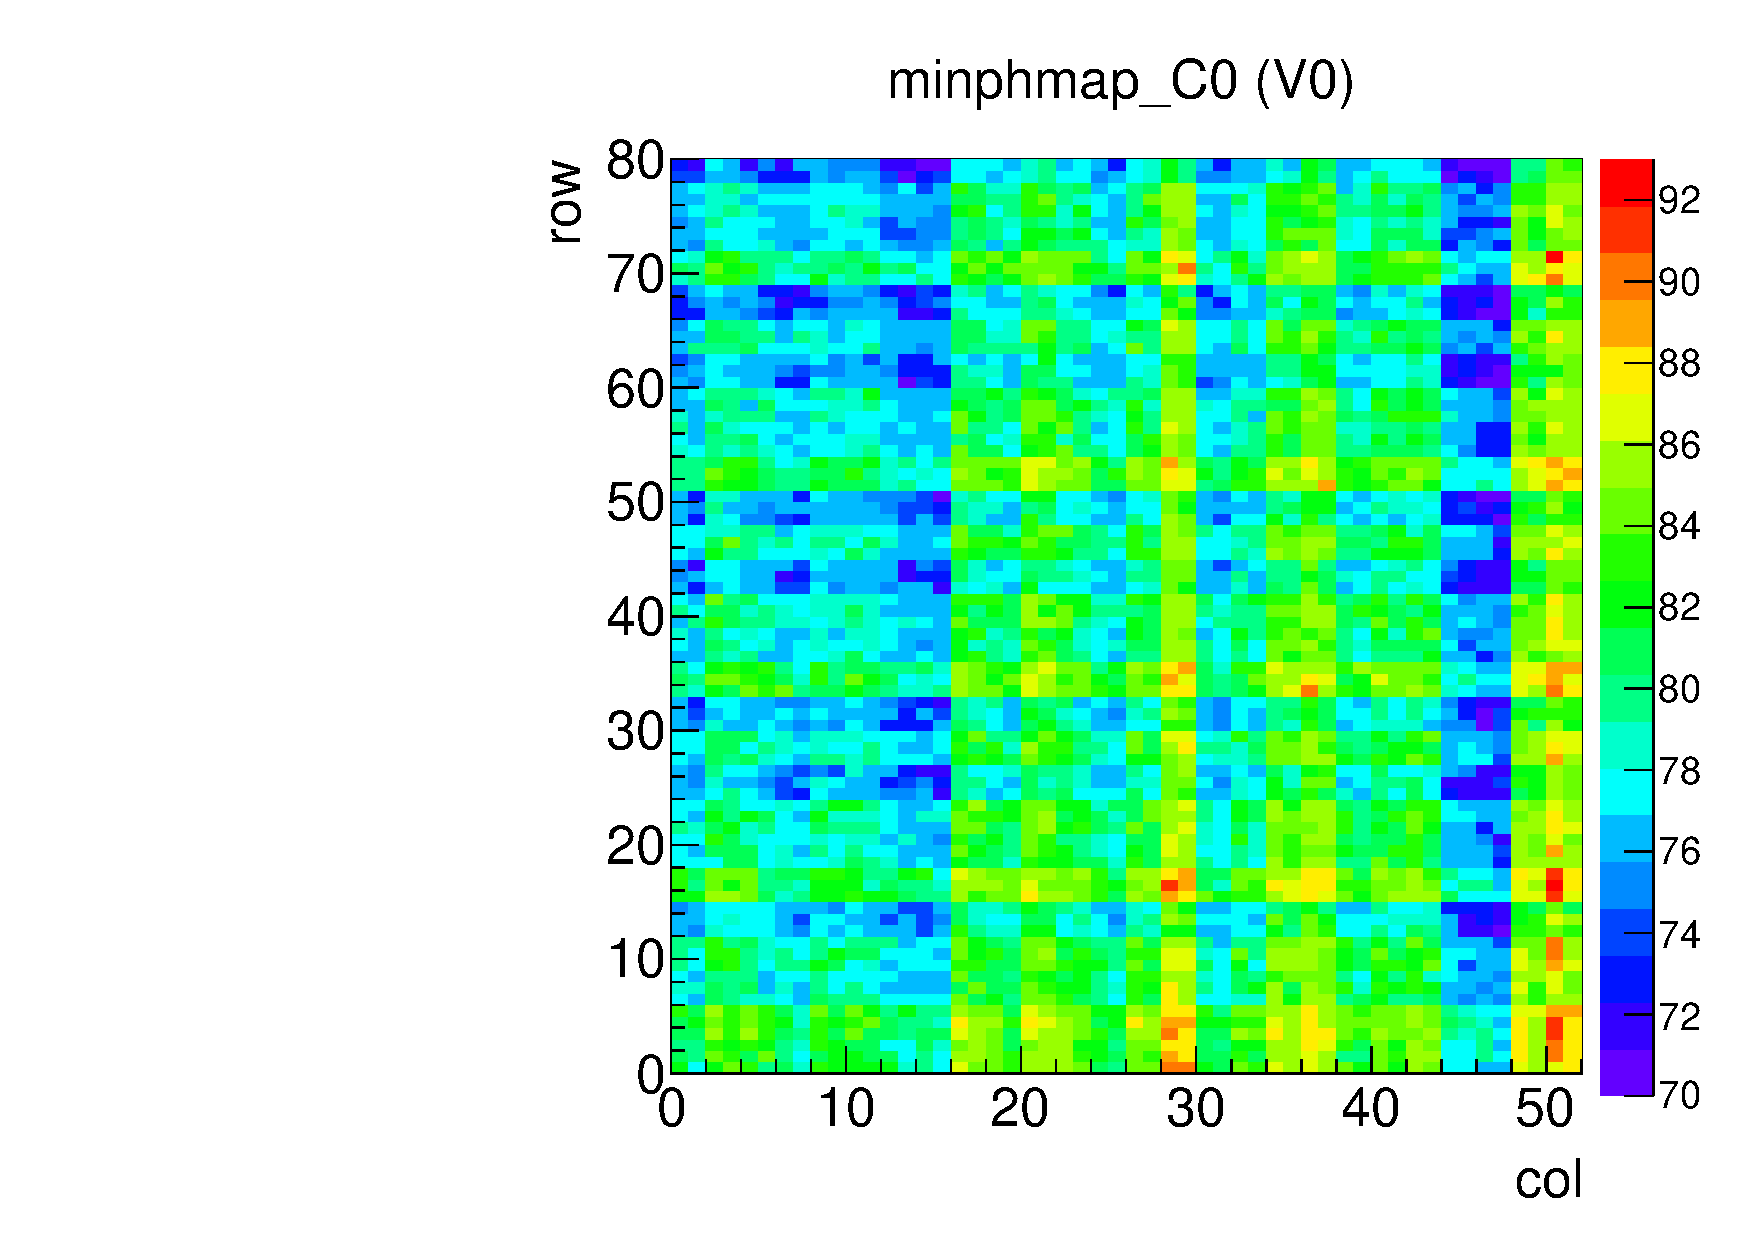
\includegraphics[width=1.0\textwidth]{figures/phopt_minphmap.pdf}
  \caption{\roc map of pulse heights with \vcal=60 (low range).}
  \label{fig:phopt_minphmap}
\end{minipage}
\hspace{0.3cm}
\begin{minipage}{0.45\textwidth}
  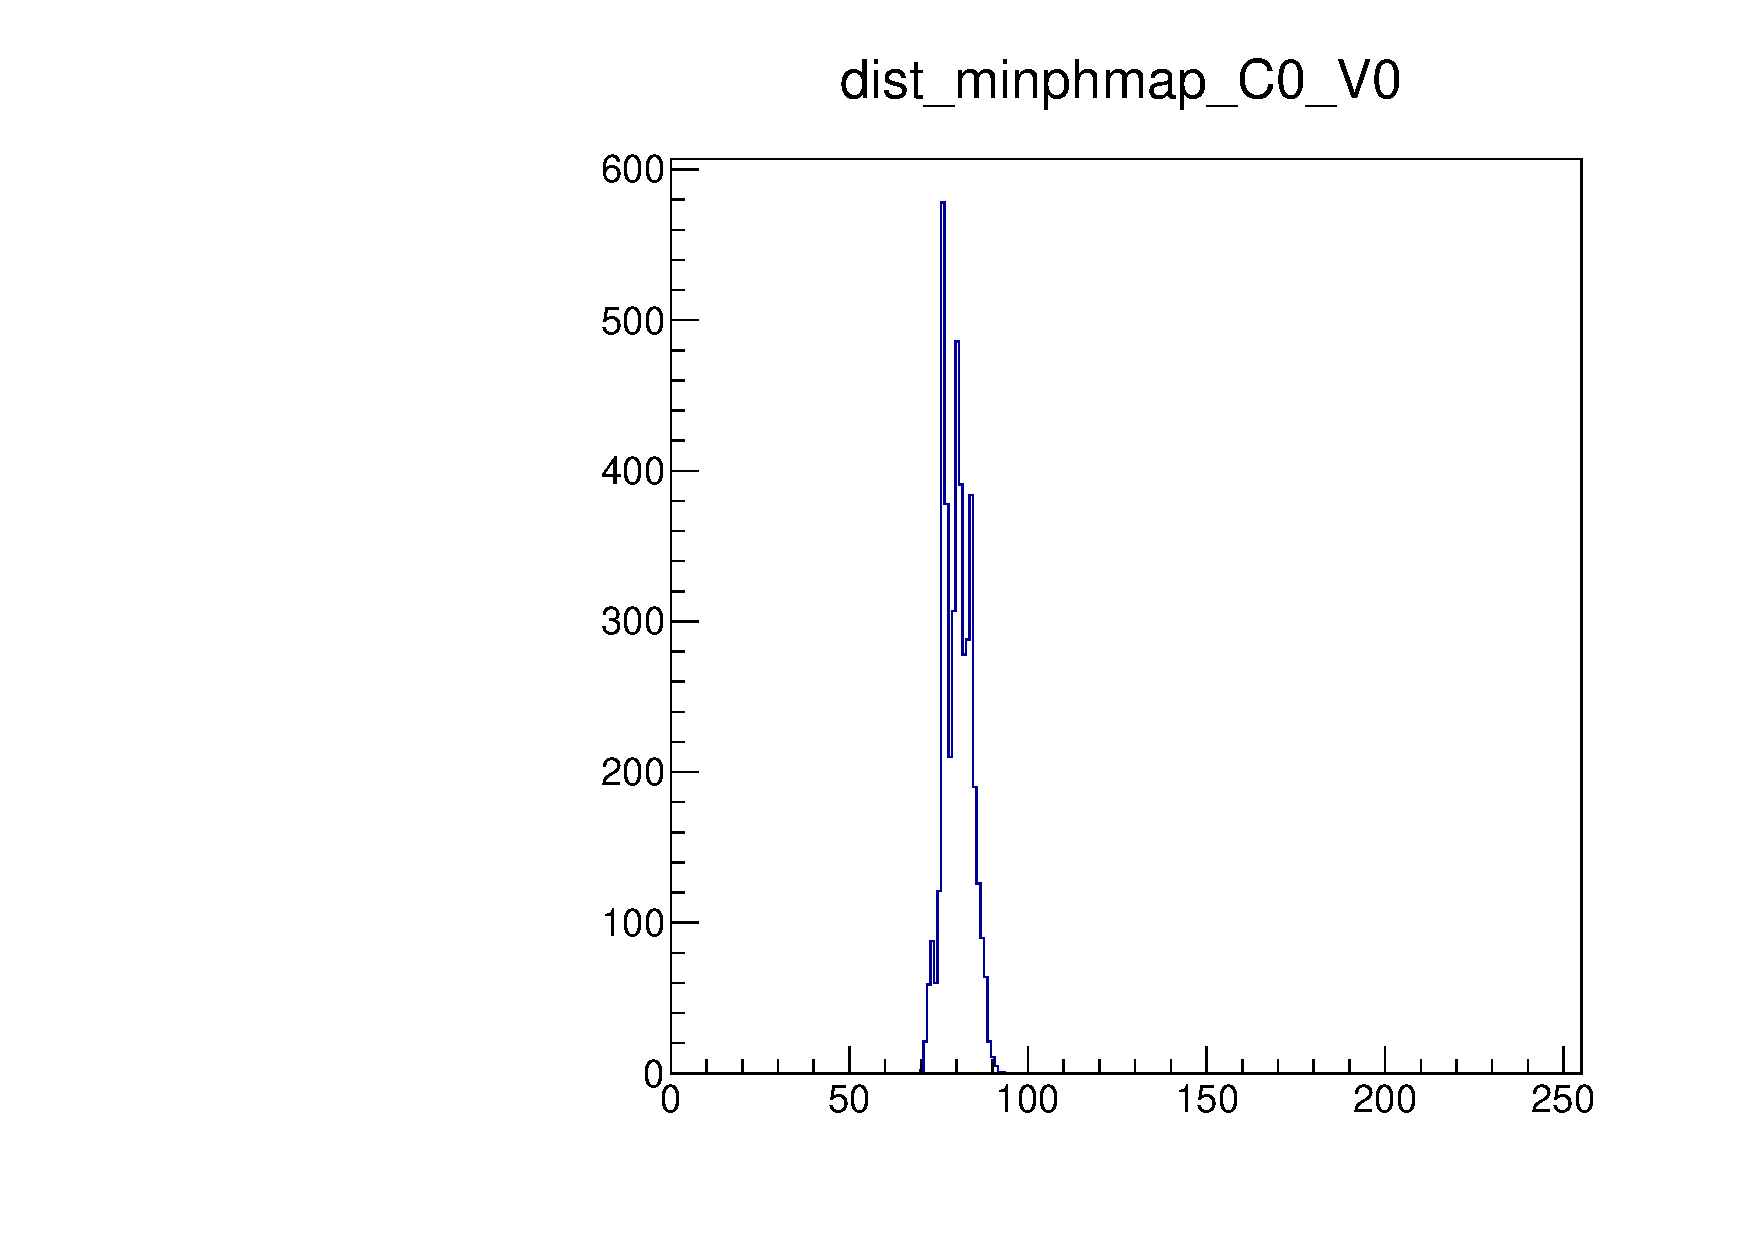
\includegraphics[width=1.0\textwidth]{figures/phopt_dist_minphmap.pdf}
  \caption{1D distribution of Figure~\ref{fig:phopt_minphmap}
           used to identify low-gain pixel.}
  \label{fig:phopt_dist_minphmap}
\end{minipage}
\end{figure}

\begin{figure}[!htp]
\centering
\begin{minipage}{0.45\textwidth}
  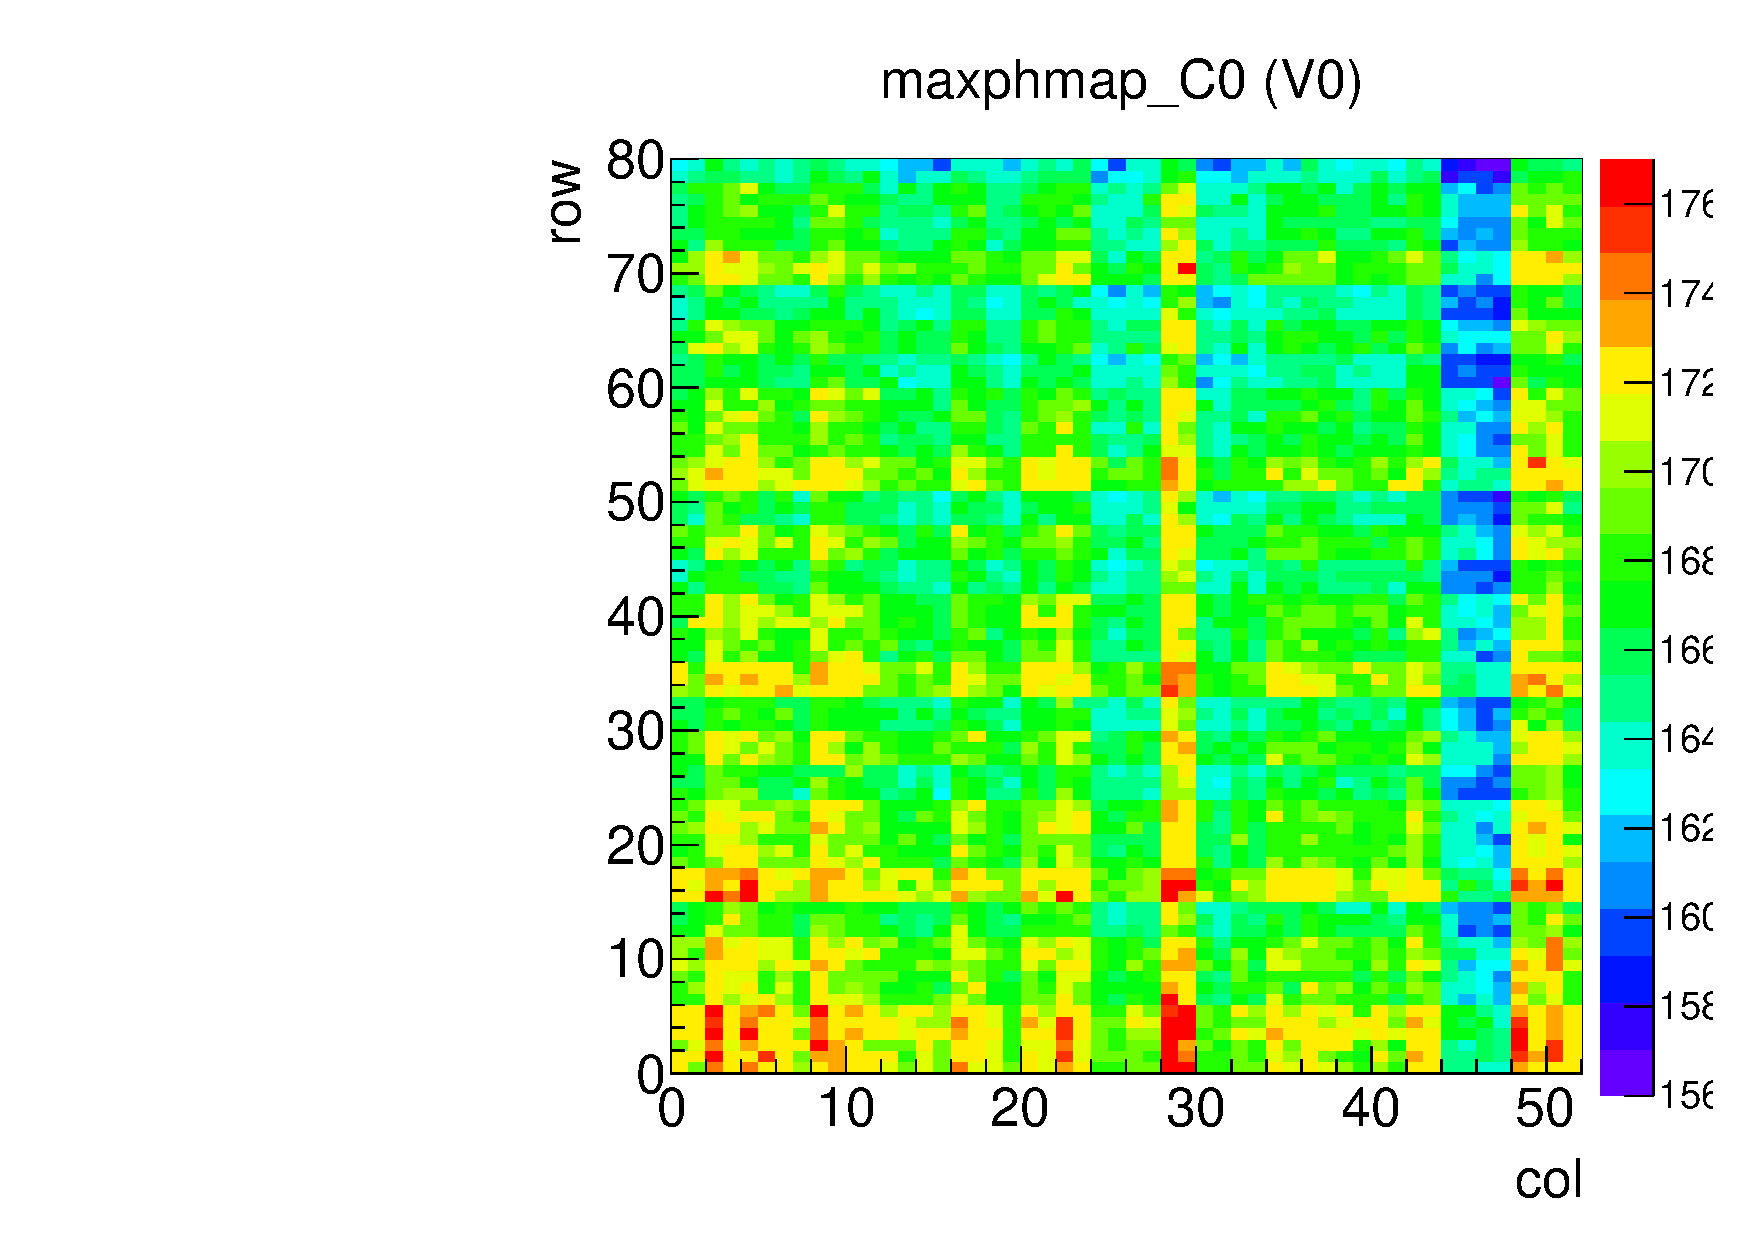
\includegraphics[width=1.0\textwidth]{figures/phopt_maxphmap.pdf}
  \caption{\roc map of pulse heights with \vcal=255 (high range).}
  \label{fig:phopt_maxphmap}
\end{minipage}
\hspace{0.3cm}
\begin{minipage}{0.45\textwidth}
  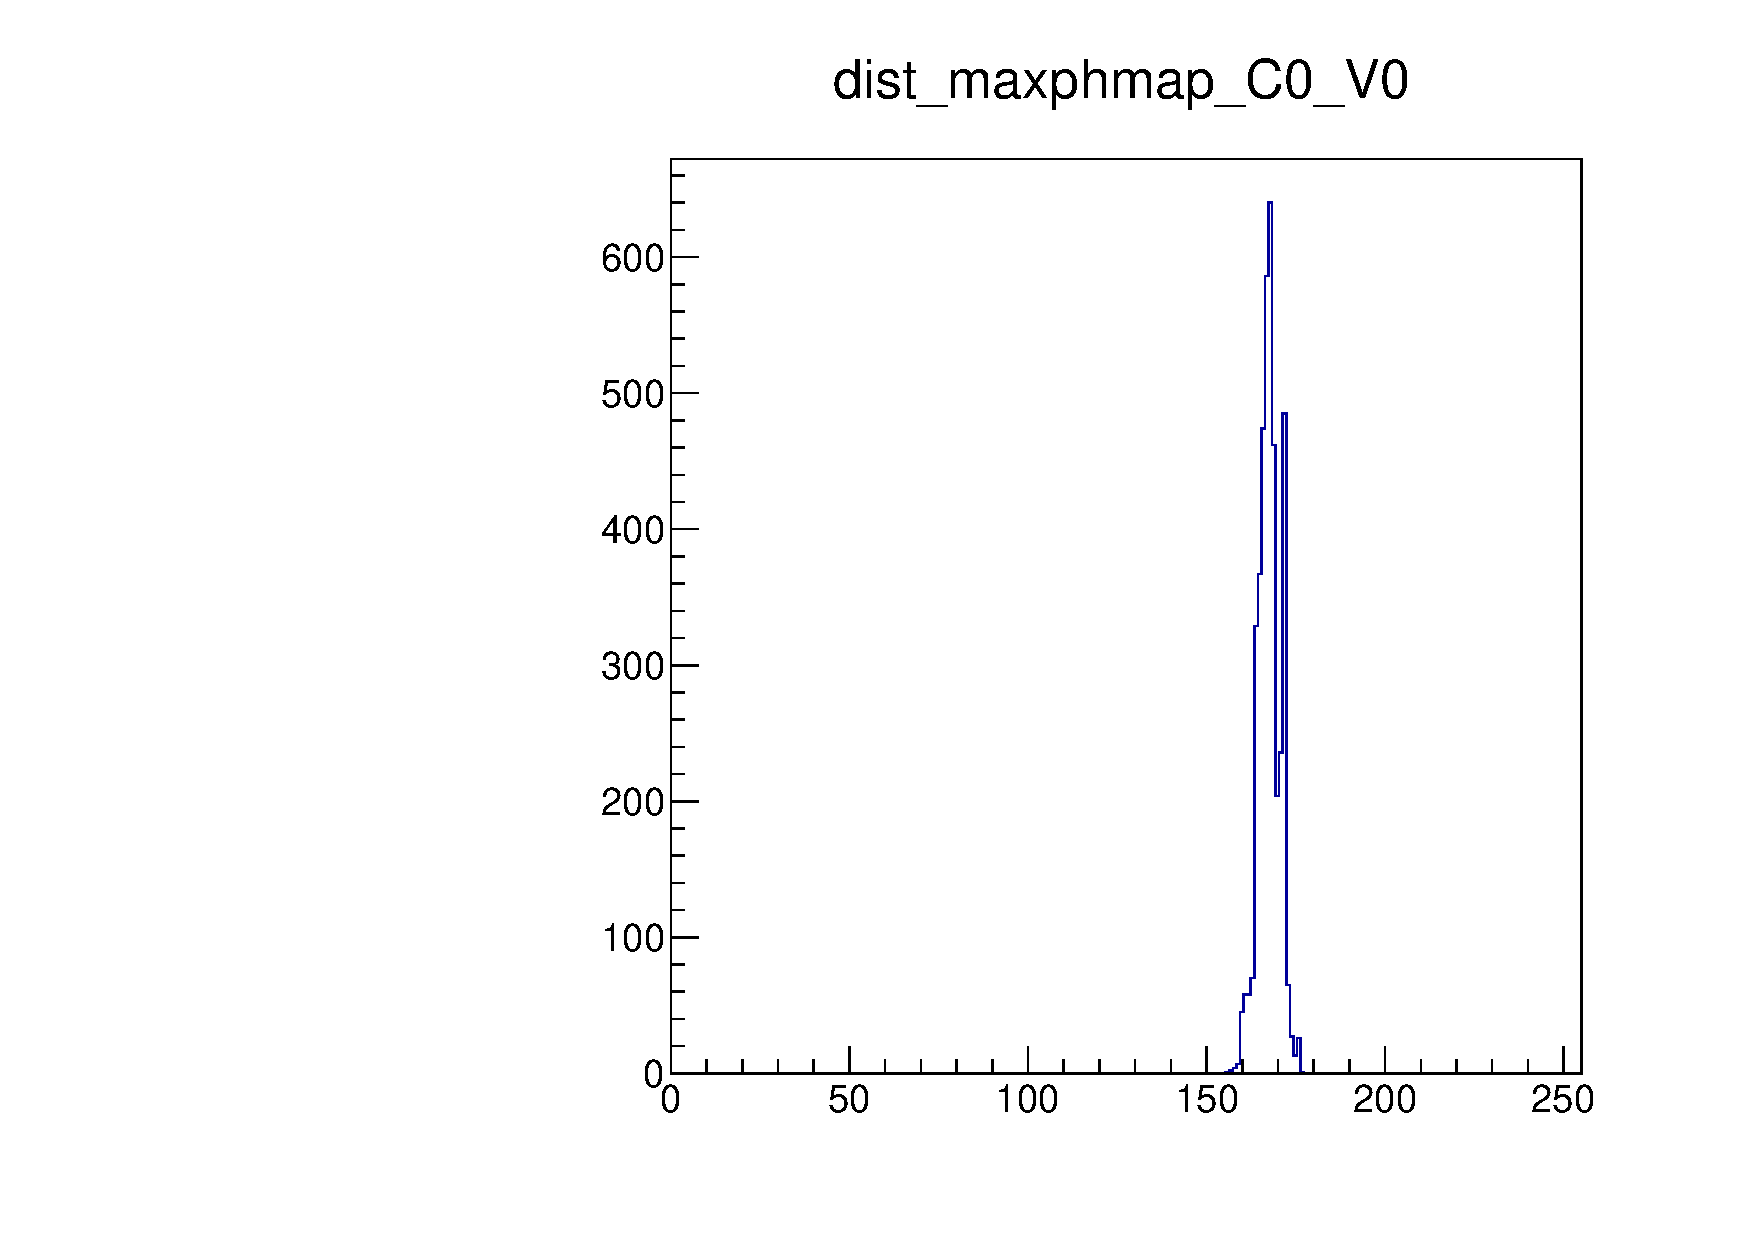
\includegraphics[width=1.0\textwidth]{figures/phopt_dist_maxphmap.pdf}
  \caption{1D distribution of Figure~\ref{fig:phopt_maxphmap}
           used to identify high-gain pixel.}
  \label{fig:phopt_dist_maxphmap}
\end{minipage}
\end{figure}

% getting maps for optimization

\begin{figure}[!htp]
\centering
\begin{minipage}{0.45\textwidth}
  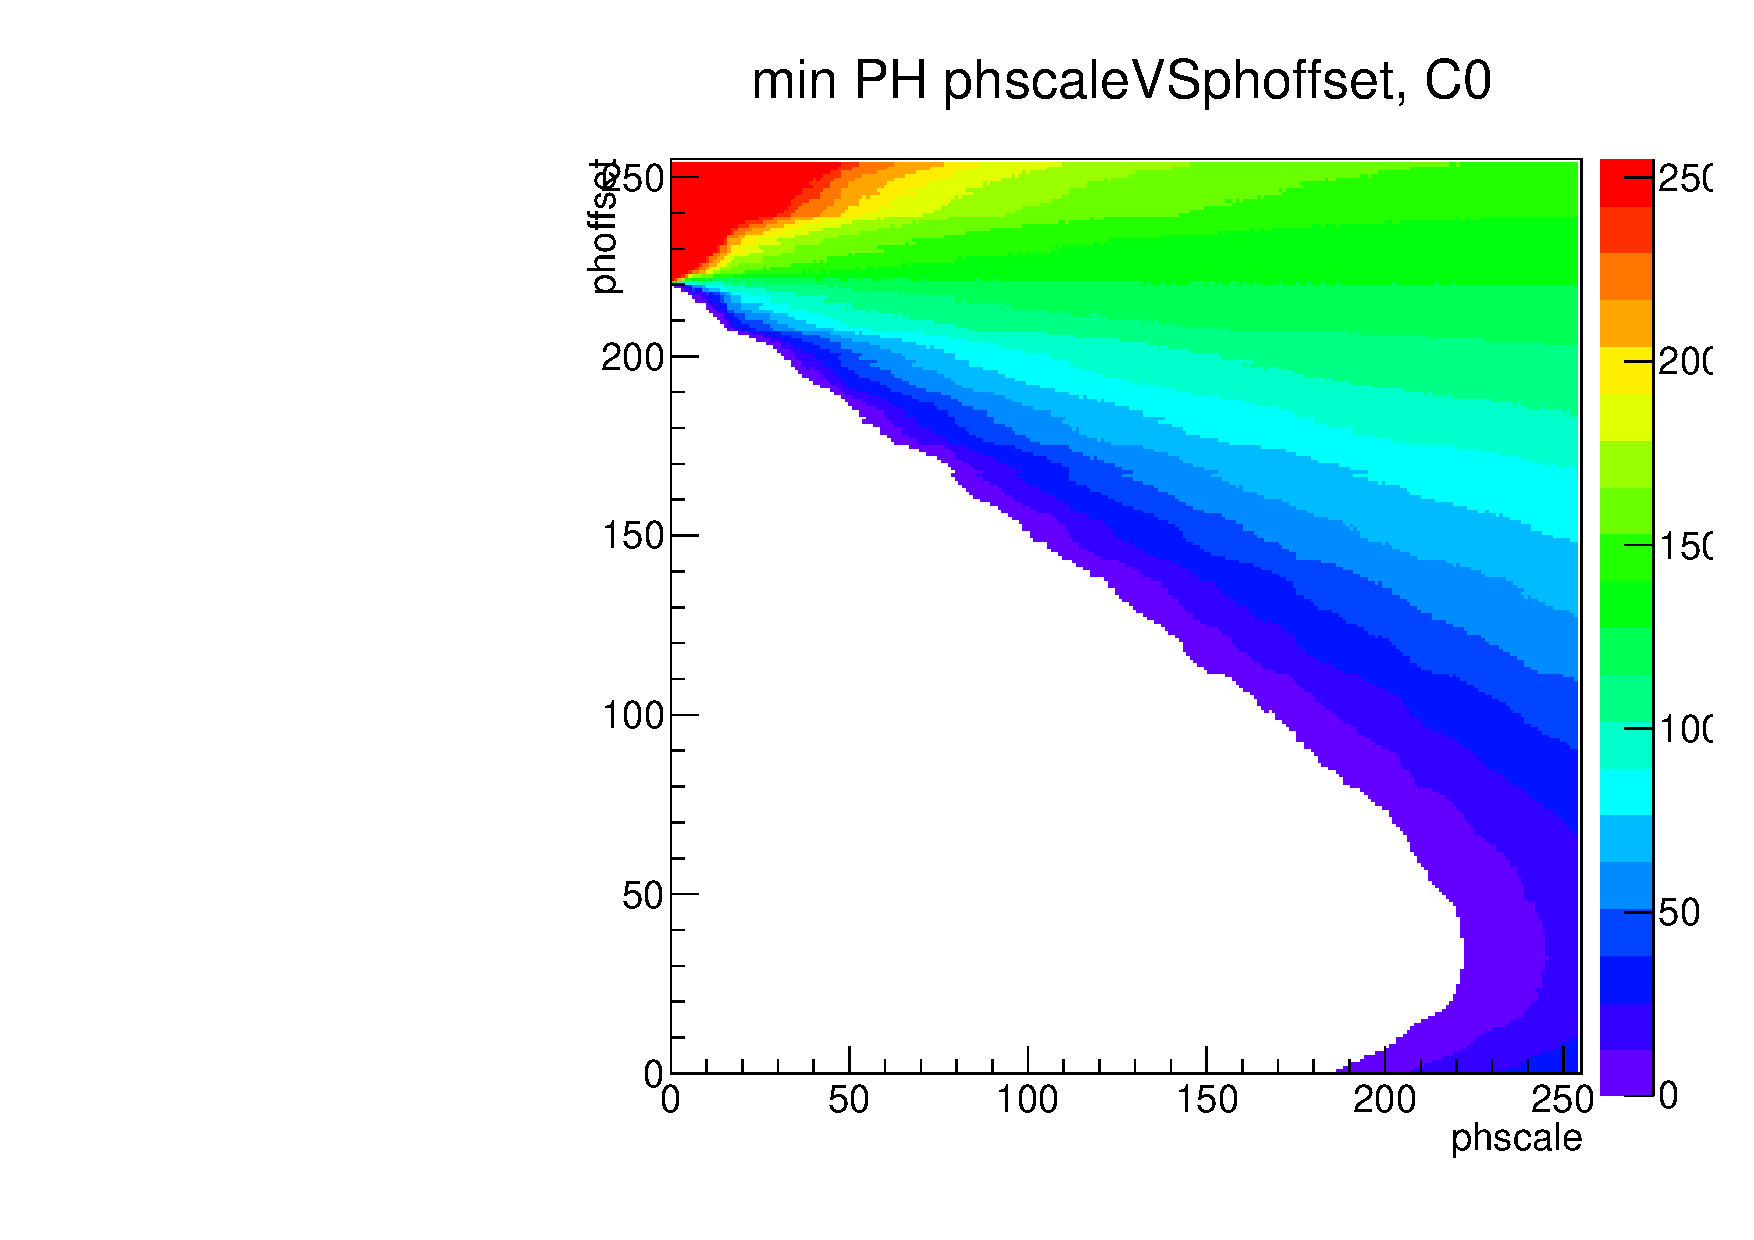
\includegraphics[width=1.0\textwidth]{figures/phopt_minphvsdacdac_th2.pdf}
  \caption{Measured PH in the \phoffset vs. \phscale plane for previously identified low-gain pixel
           with minimum \vcal required to fire the pixel.}
  \label{fig:phopt_minphvsdacdac_th2}
\end{minipage}
\hspace{0.3cm}
\begin{minipage}{0.45\textwidth}
  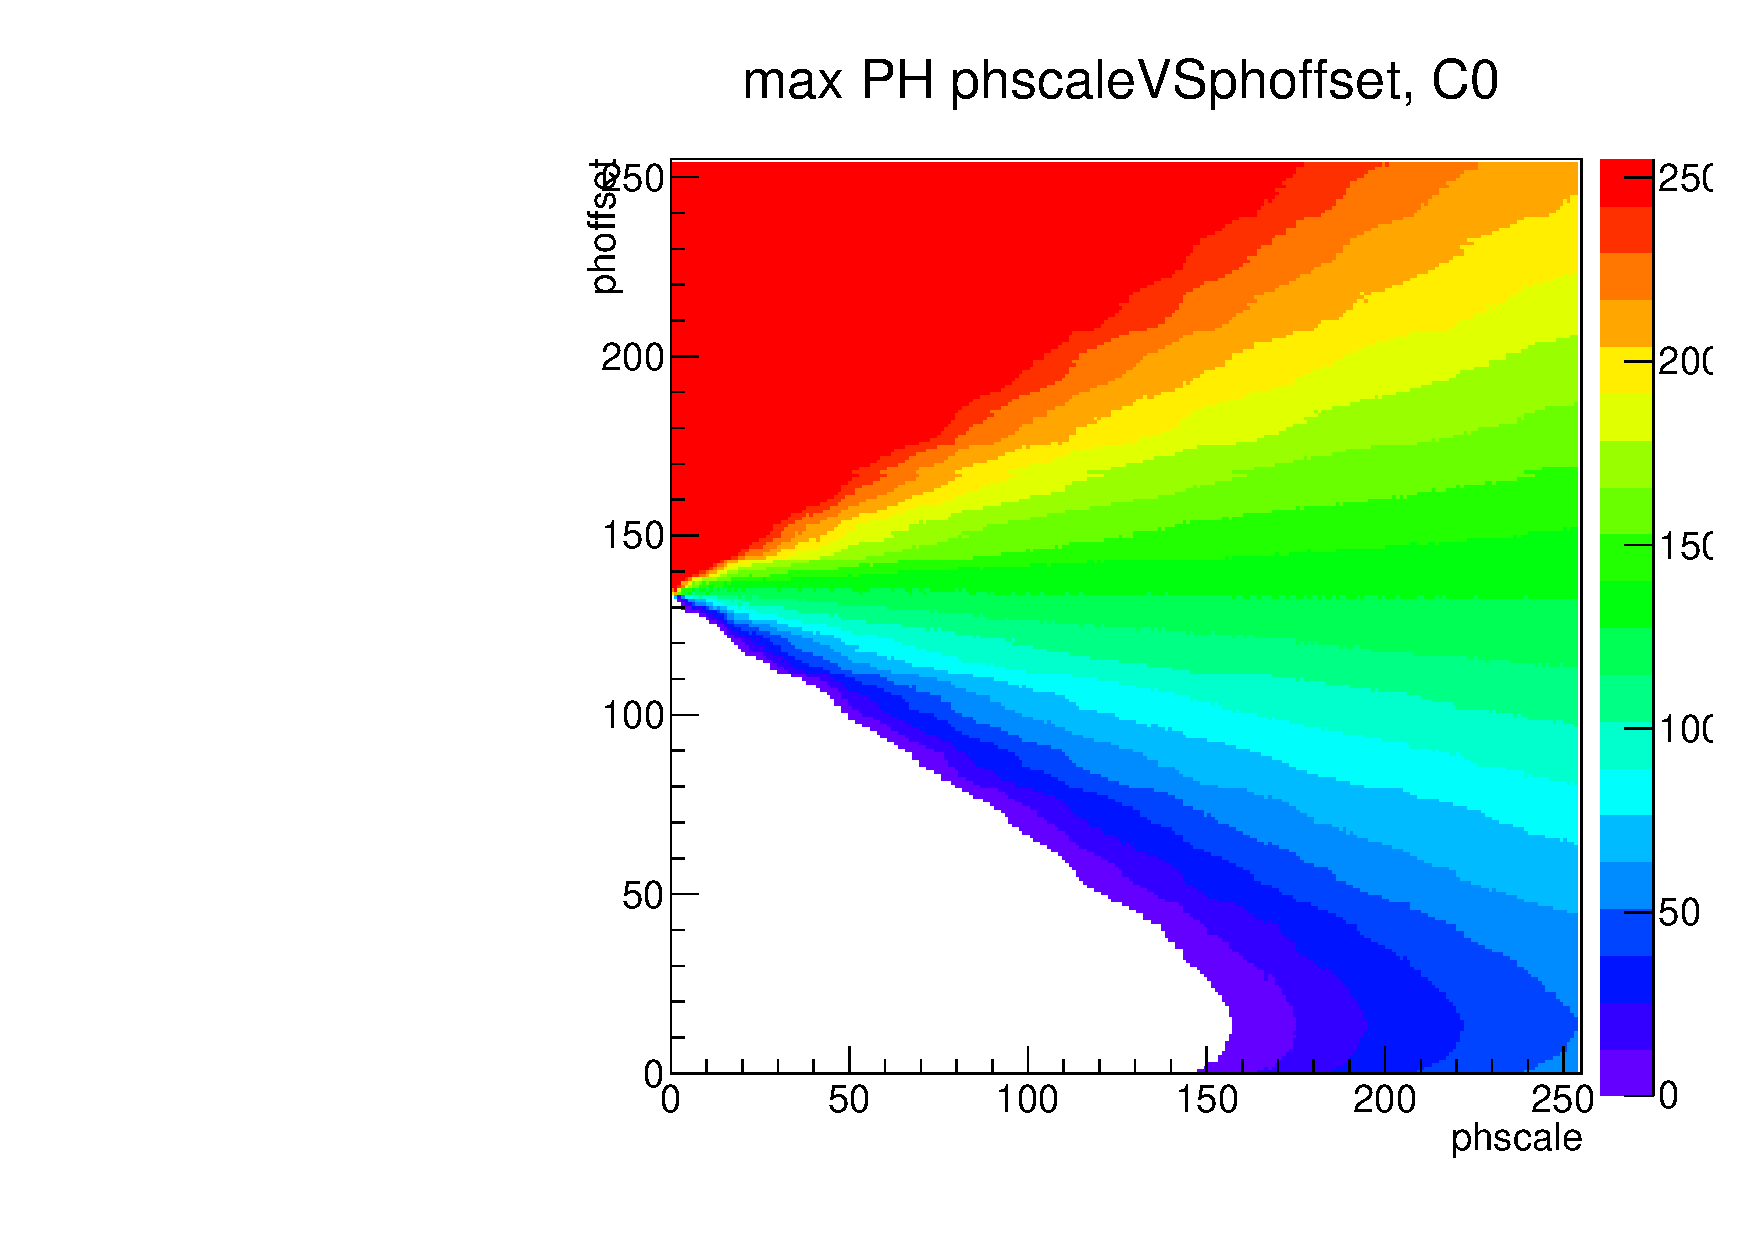
\includegraphics[width=1.0\textwidth]{figures/phopt_maxphvsdacdac_th2.pdf}
  \caption{Measured PH in the \phoffset vs. \phscale plane for previously identified high-gain pixel
           with \vcal set to the chosen ADC saturation point.}
  \label{fig:phopt_maxphvsdacdac_th2}
\end{minipage}
\end{figure}

\begin{figure}[!htp]
\centering
\begin{minipage}{0.45\textwidth}
  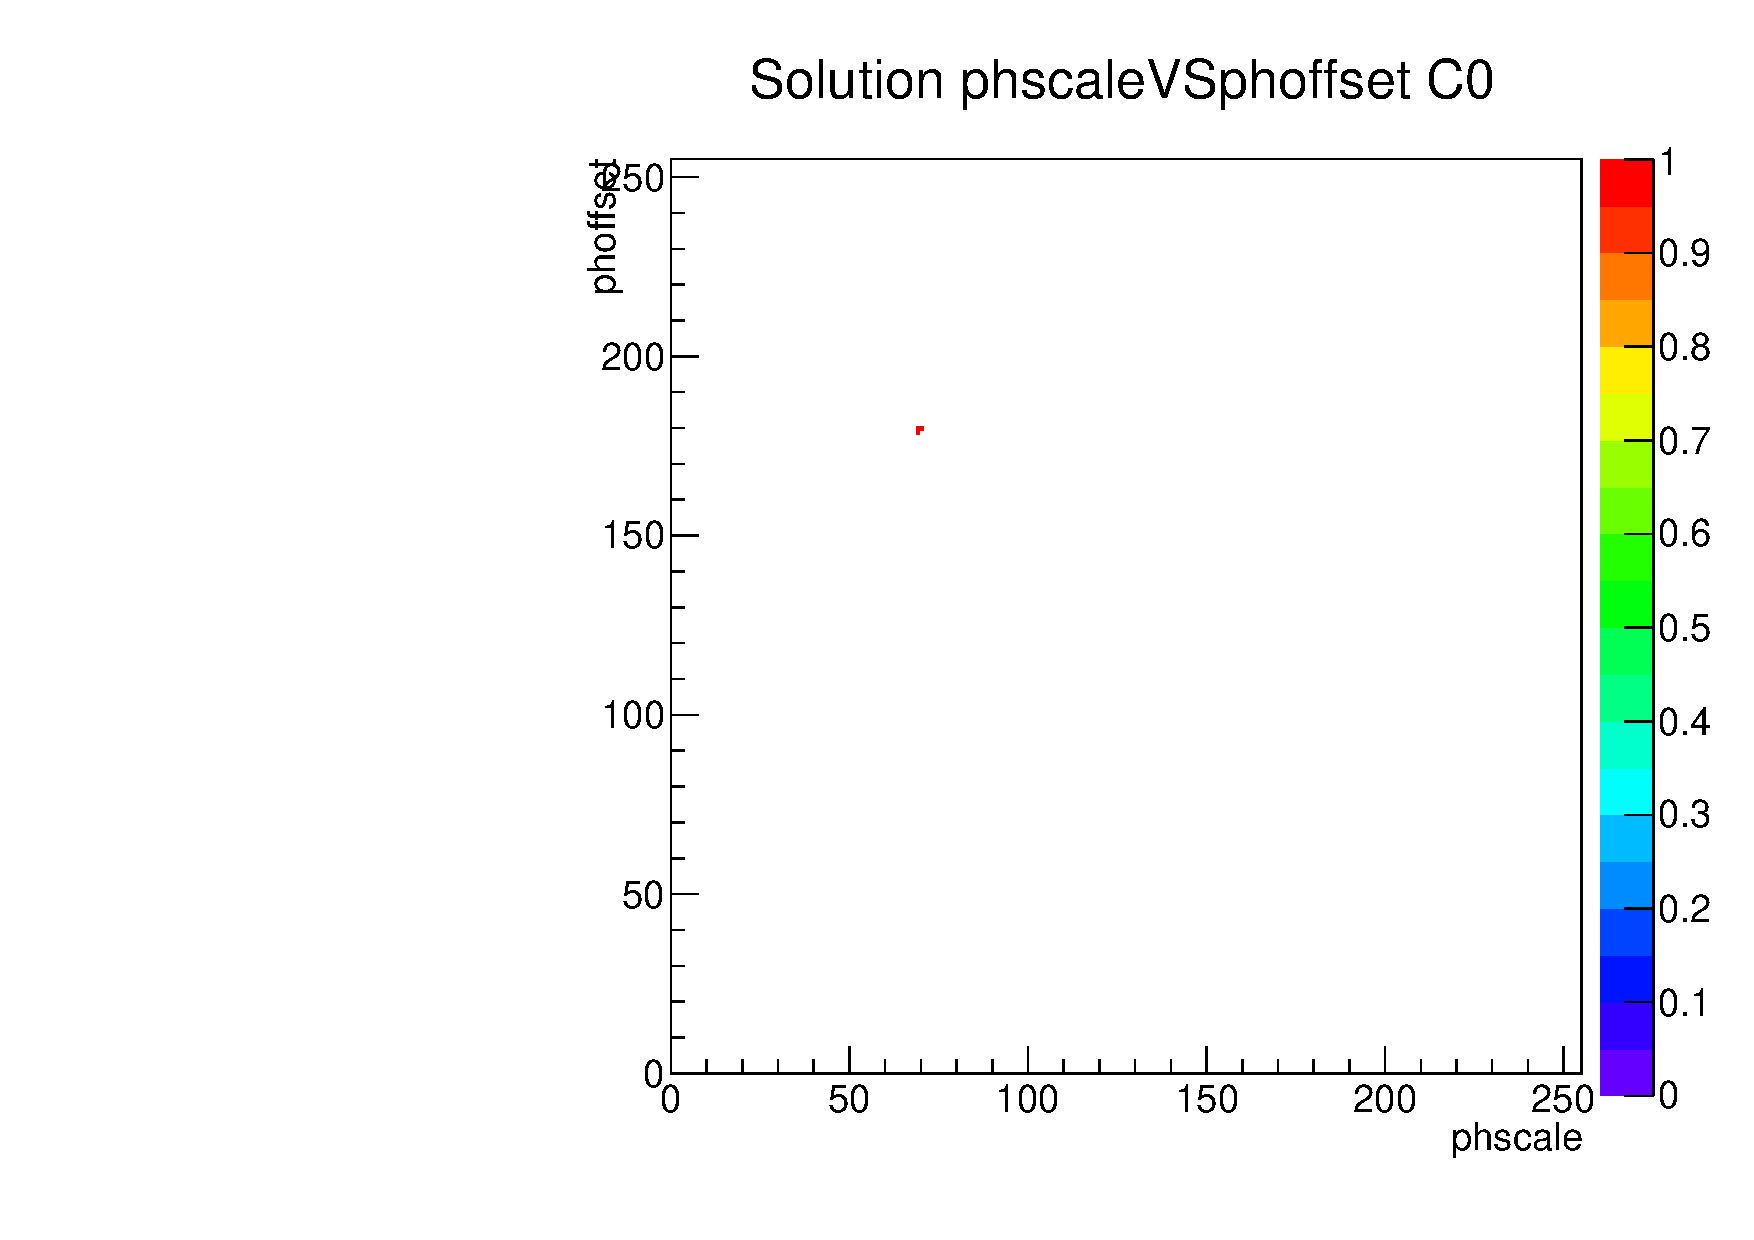
\includegraphics[width=1.0\textwidth]{figures/phopt_solphvsdacdac_th2.pdf}
  \caption{Overlap of optimal regimes in Figures~\ref{fig:phopt_minphvsdacdac_th2} and~\ref{fig:phopt_maxphvsdacdac_th2}.
           A red entry signifies an optimal pair of \phoffset and \phscale values.}
  \label{fig:phopt_solphvsdacdac_th2}
\end{minipage}
\end{figure}

% gain plots for highest/lowest gain pixels with optimized DACs

\begin{figure}[!htp]
\centering
\begin{minipage}{0.45\textwidth}
  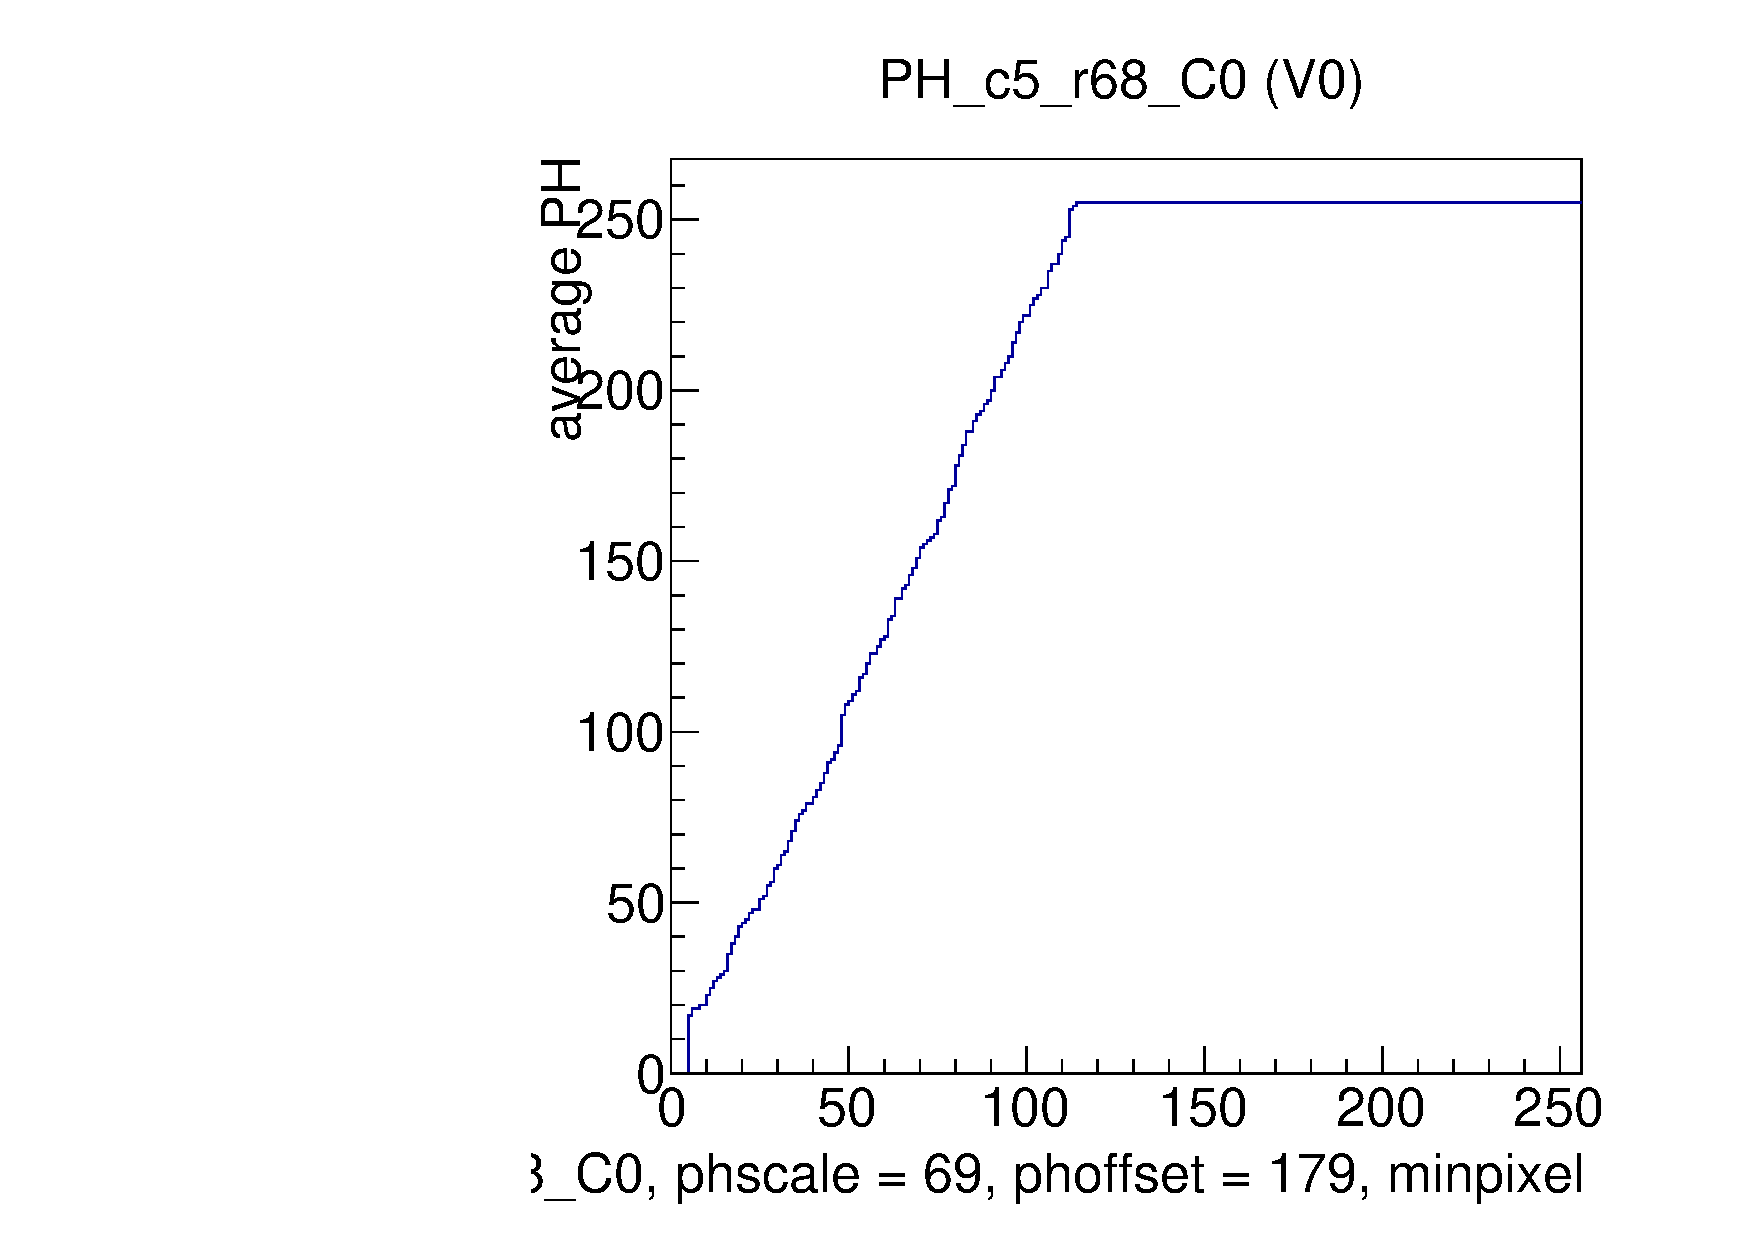
\includegraphics[width=1.0\textwidth]{figures/phopt_PH_c5_r68.pdf}
  \caption{PH vs.~(high-range)  \vcal curve for previously identified low-gain pixel.}
  \label{fig:phopt_PH_c5_r68}
\end{minipage}
\hspace{0.3cm}
\begin{minipage}{0.45\textwidth}
  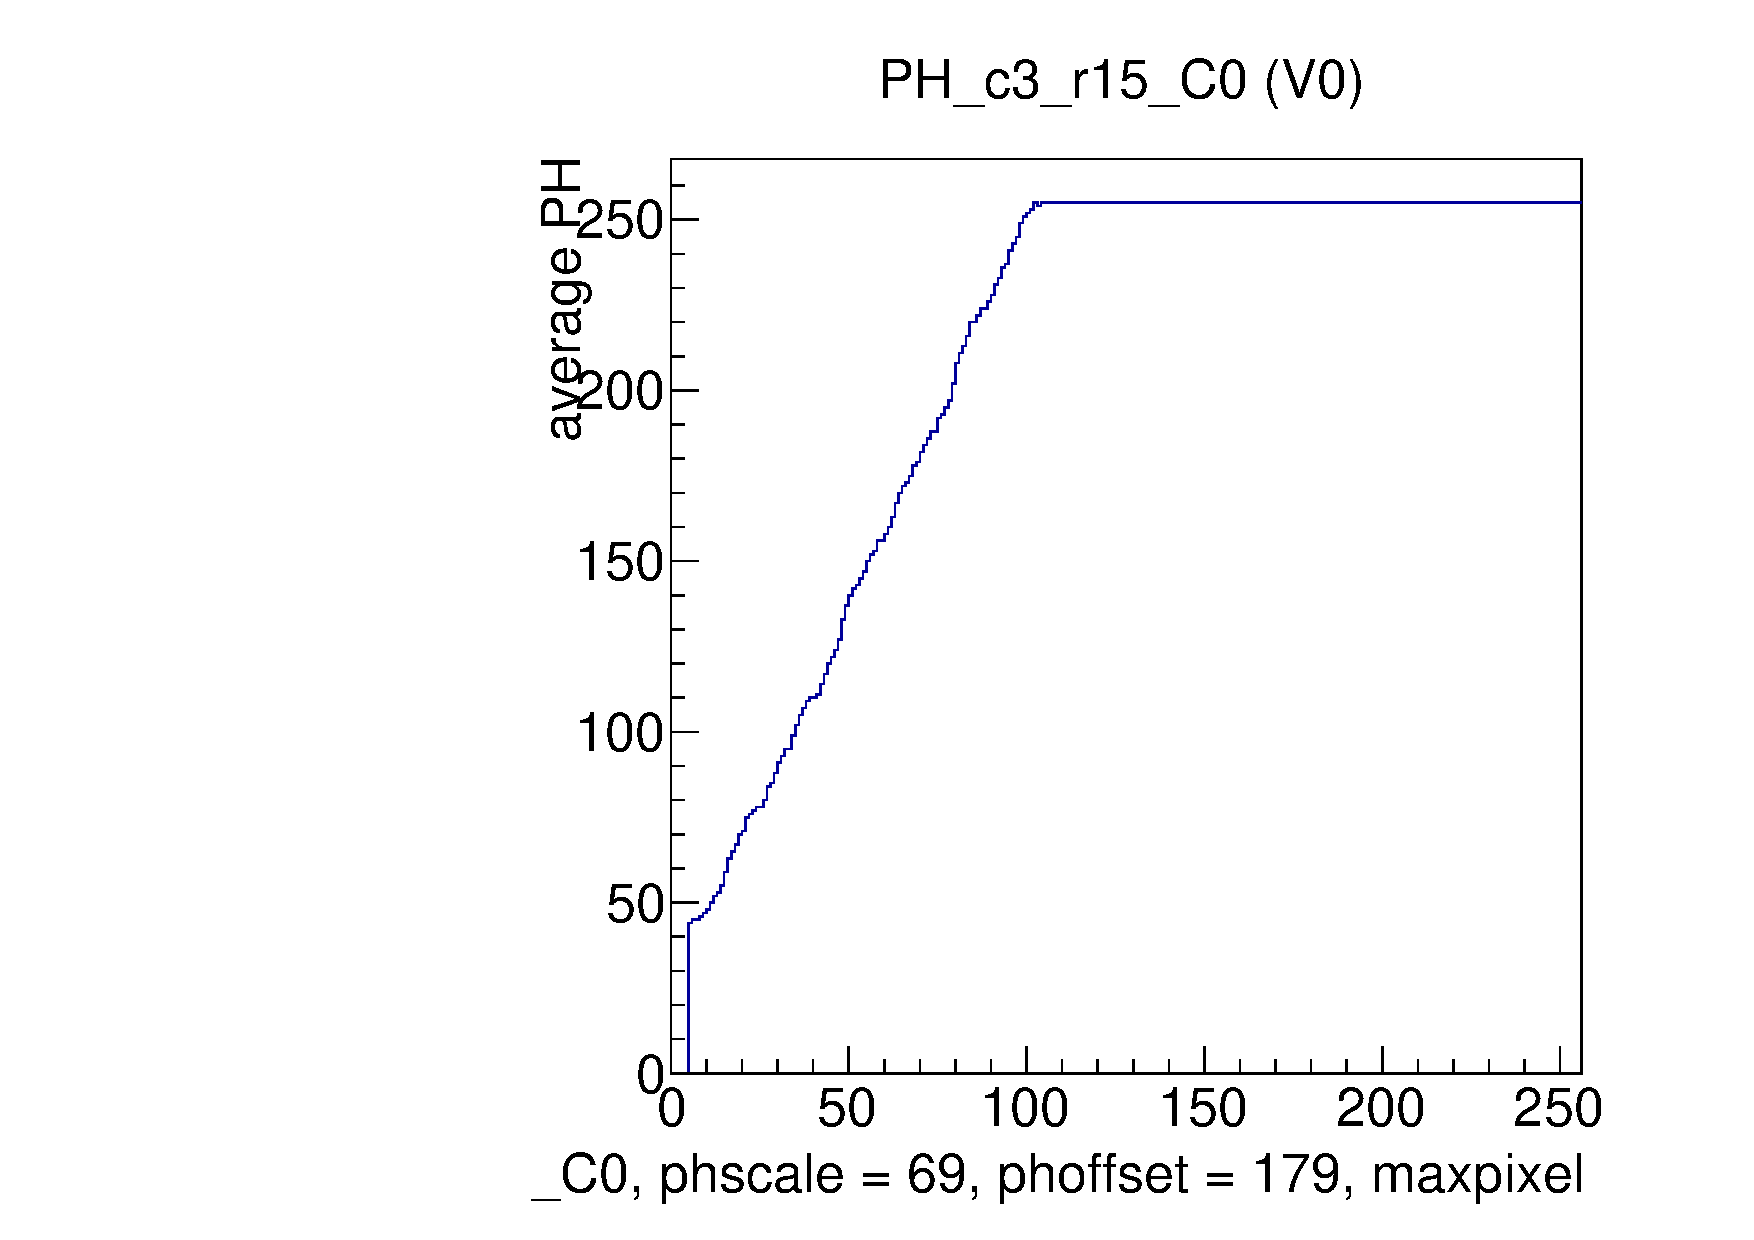
\includegraphics[width=1.0\textwidth]{figures/phopt_PH_c3_r15.pdf}
  \caption{PH vs.~(high-range) \vcal curve for previously identified high-gain pixel.}
  \label{fig:phopt_PH_c3_r15}
\end{minipage}
\end{figure}


% doing scans at three points in vcal

% done with Vcal set 10 units above turn-on for least sensitive pixel

\begin{figure}[!htp]
\centering
\begin{minipage}{0.45\textwidth}
  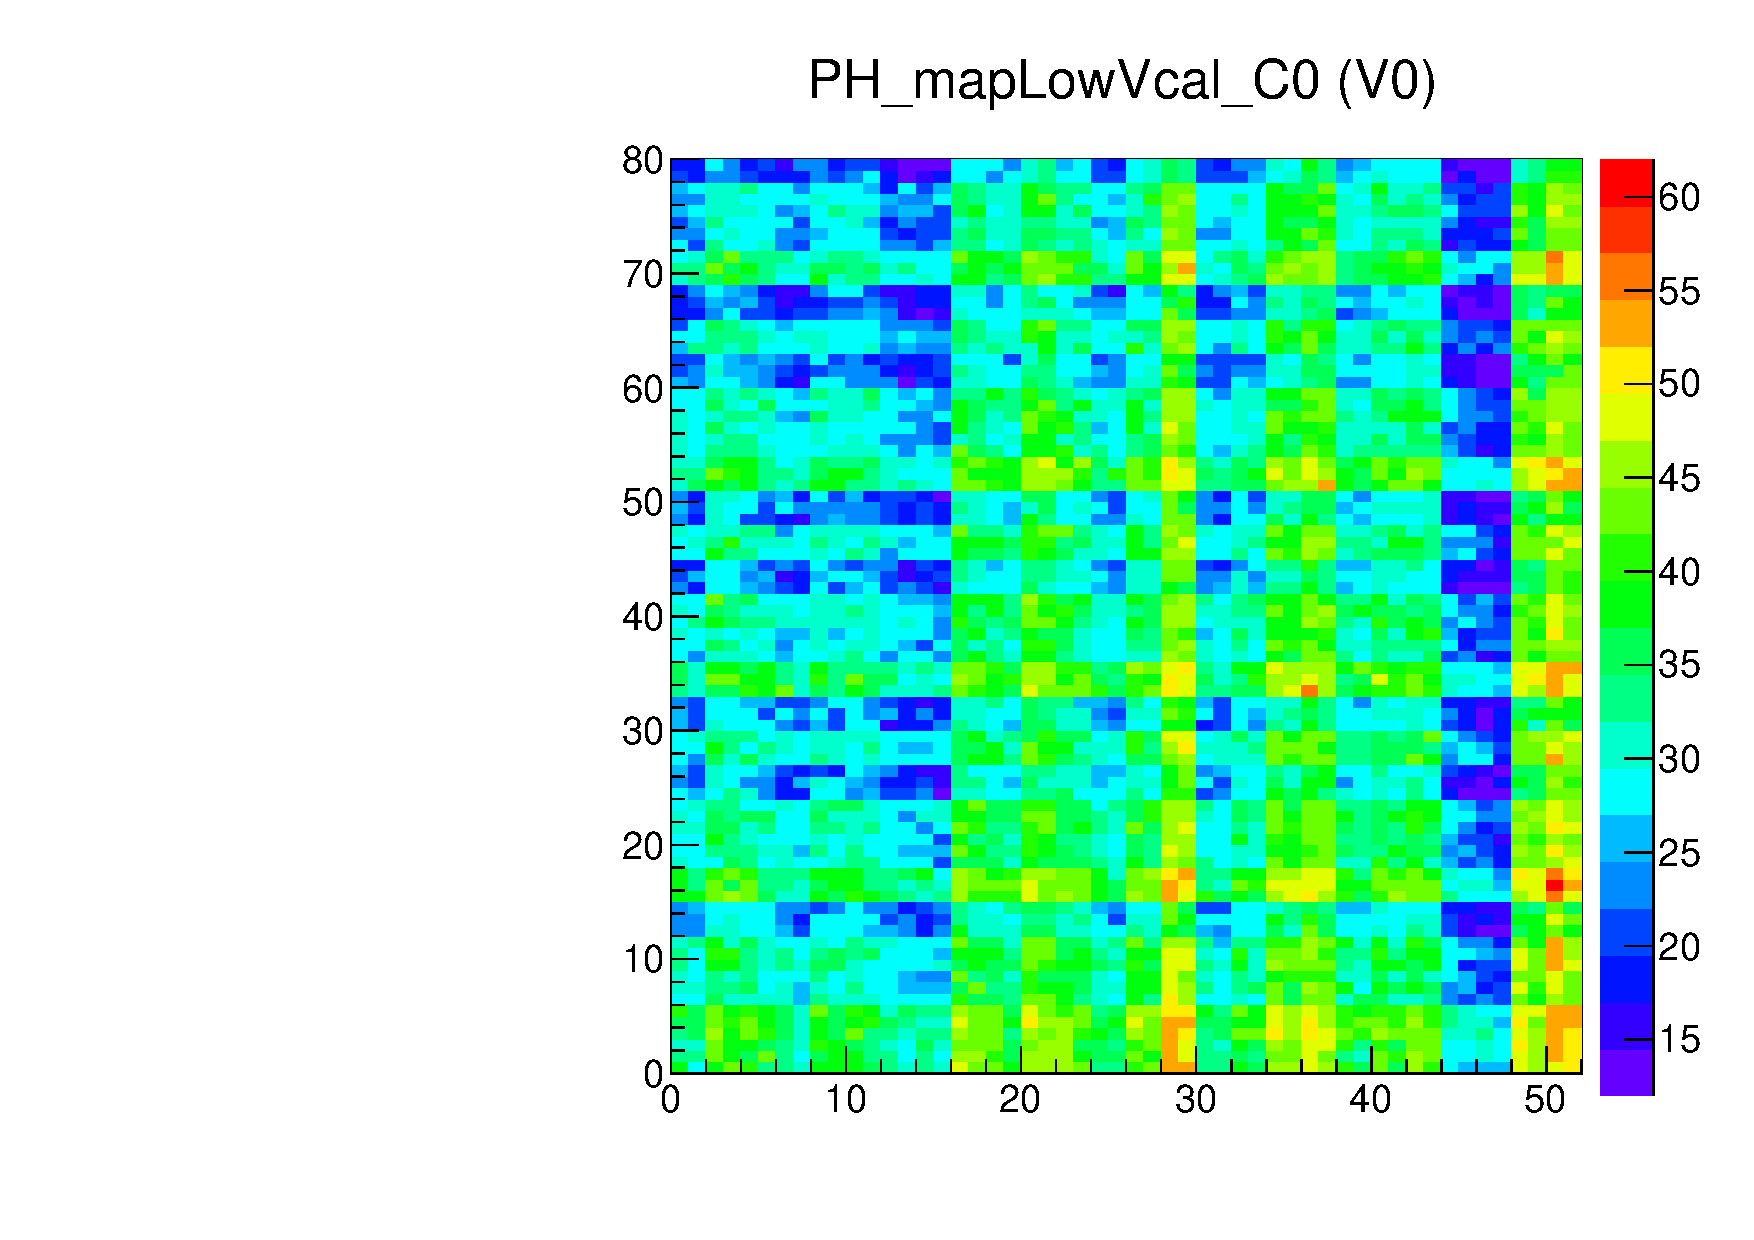
\includegraphics[width=1.0\textwidth]{figures/phopt_PH_mapLowVcal.pdf}
  \caption{\roc map of pulse heights with \vcal 10 units above minimum \vcal for low-gain pixel.}
  \label{fig:phopt_PH_mapLowVcal}
\end{minipage}
\hspace{0.3cm}
\begin{minipage}{0.45\textwidth}
  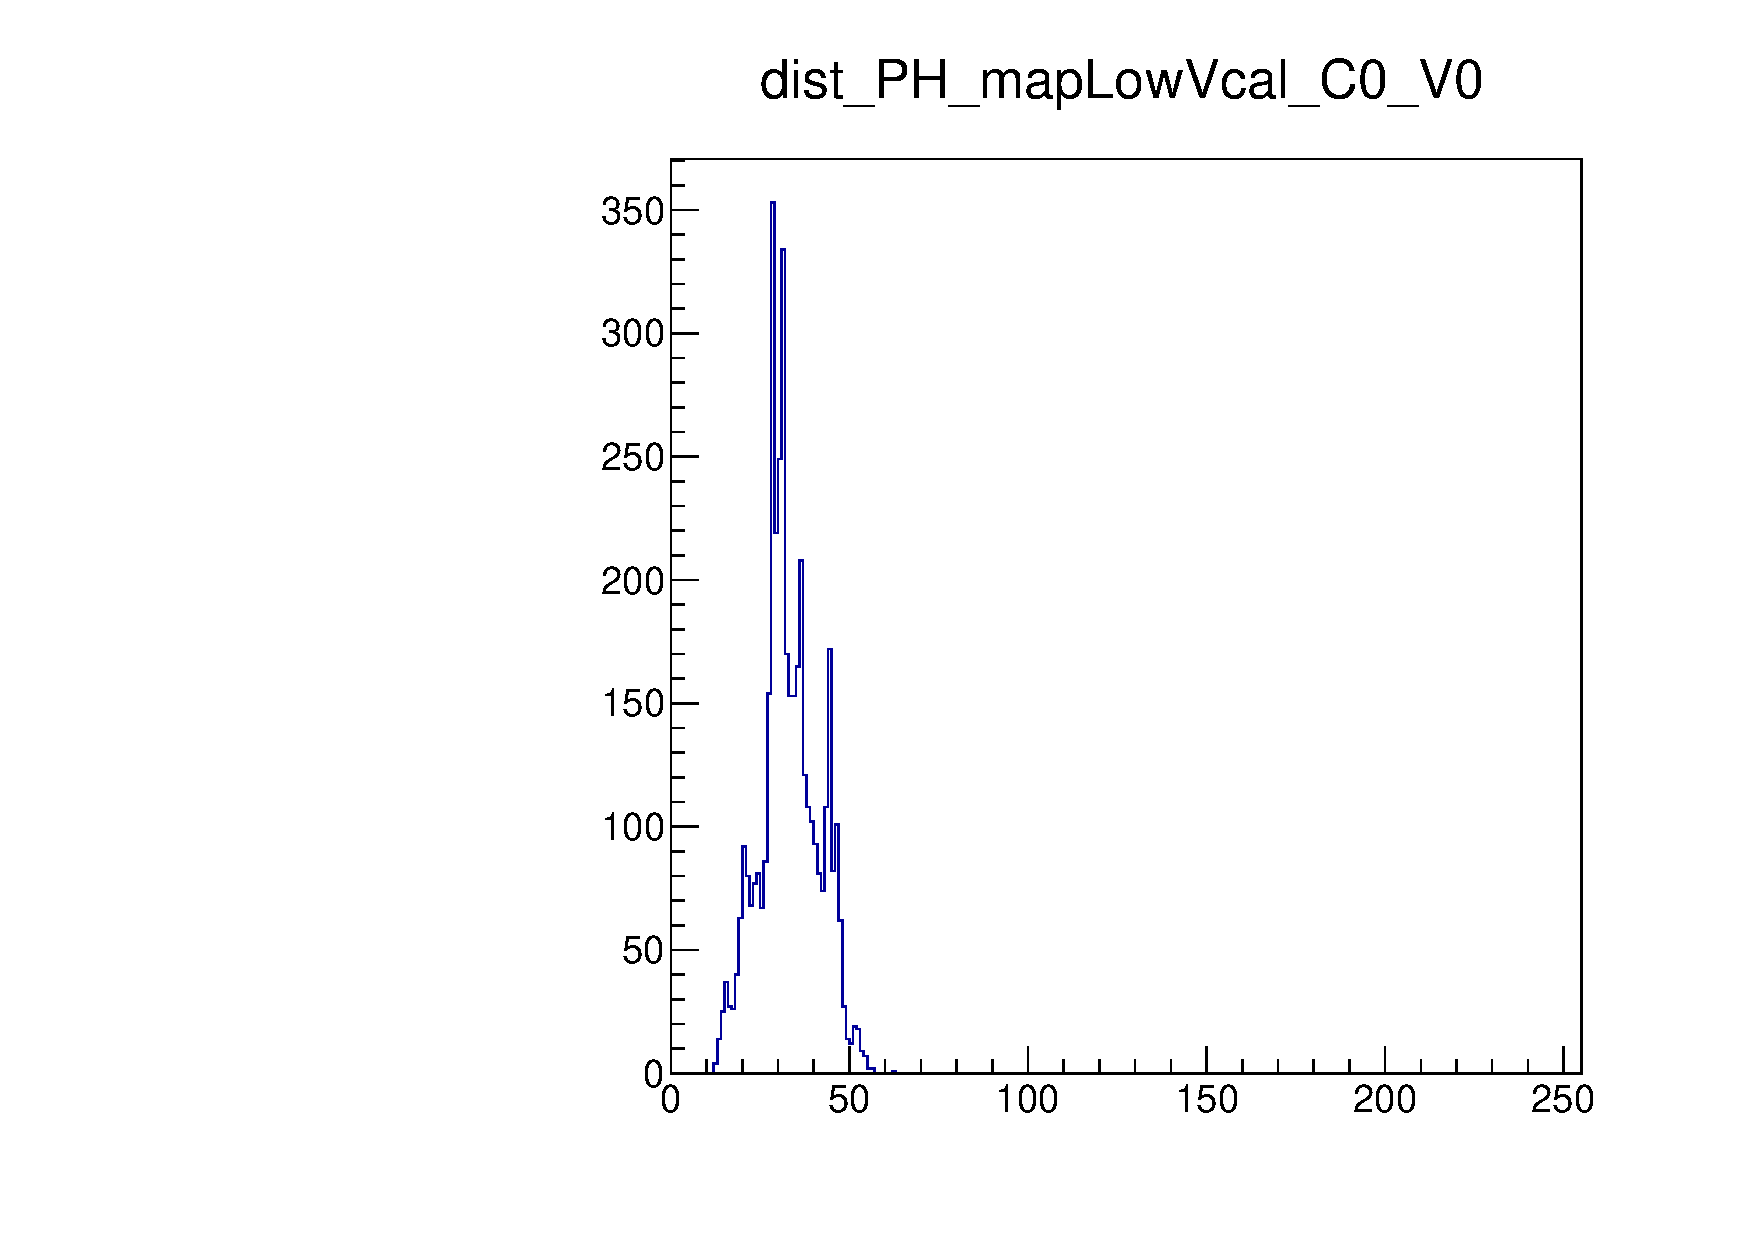
\includegraphics[width=1.0\textwidth]{figures/phopt_dist_PH_mapLowVcal.pdf}
  \caption{1D distribution of Figure~\ref{fig:phopt_PH_mapLowVcal}.}
  \label{fig:phopt_dist_PH_mapLowVcal}
\end{minipage}
\end{figure}

\begin{figure}[!htp]
\centering
\begin{minipage}{0.45\textwidth}
  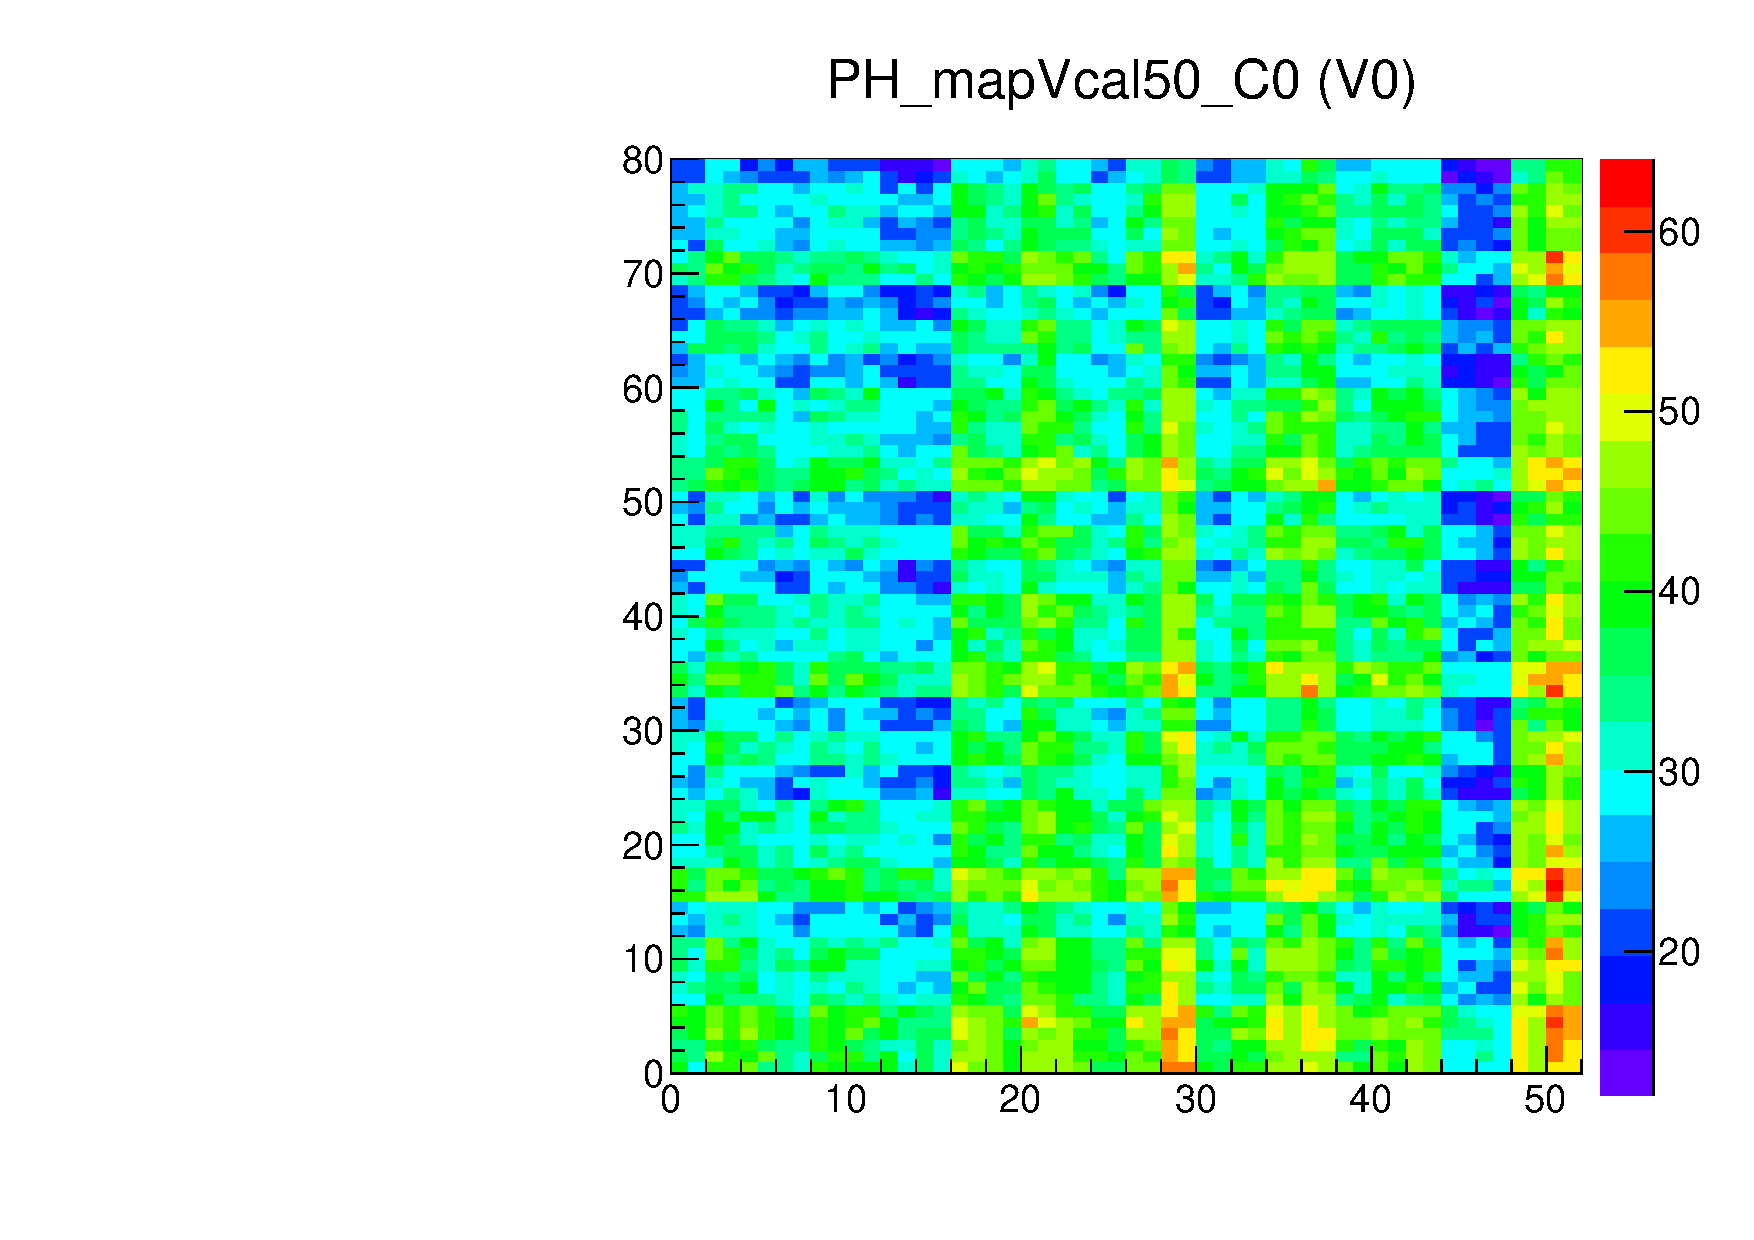
\includegraphics[width=1.0\textwidth]{figures/phopt_PH_mapVcal50.pdf}
  \caption{\roc map of pulse heights with \vcal=50 (low range).}
  \label{fig:phopt_PH_mapVcal50}
\end{minipage}
\hspace{0.3cm}
\begin{minipage}{0.45\textwidth}
  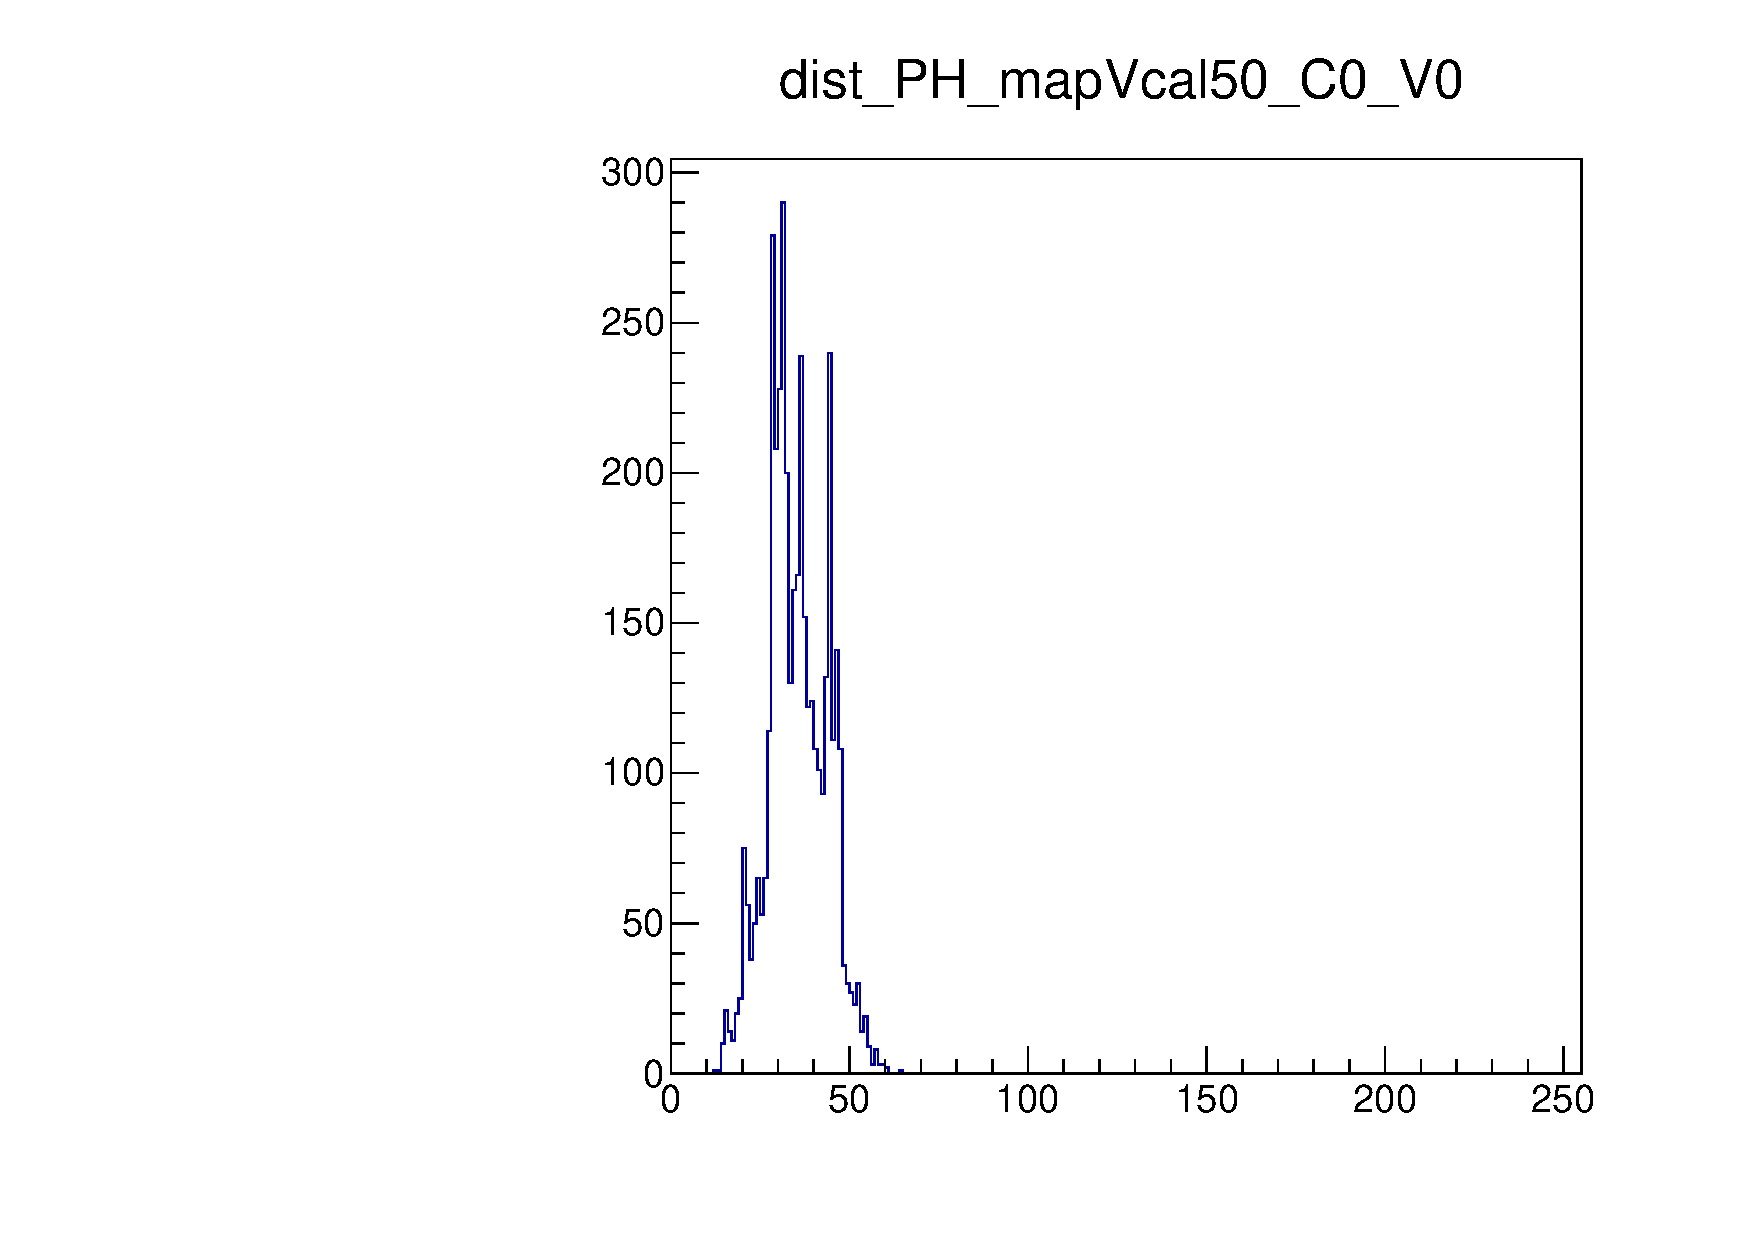
\includegraphics[width=1.0\textwidth]{figures/phopt_dist_PH_mapVcal50.pdf}
  \caption{1D distribution of Figure~\ref{fig:phopt_PH_mapVcal50}.}
  \label{fig:phopt_dist_PH_mapVcal50}
\end{minipage}
\end{figure}

% done at user-defined target saturation Vcal - default 100 (high range)

\begin{figure}[!htp]
\centering
\begin{minipage}{0.45\textwidth}
  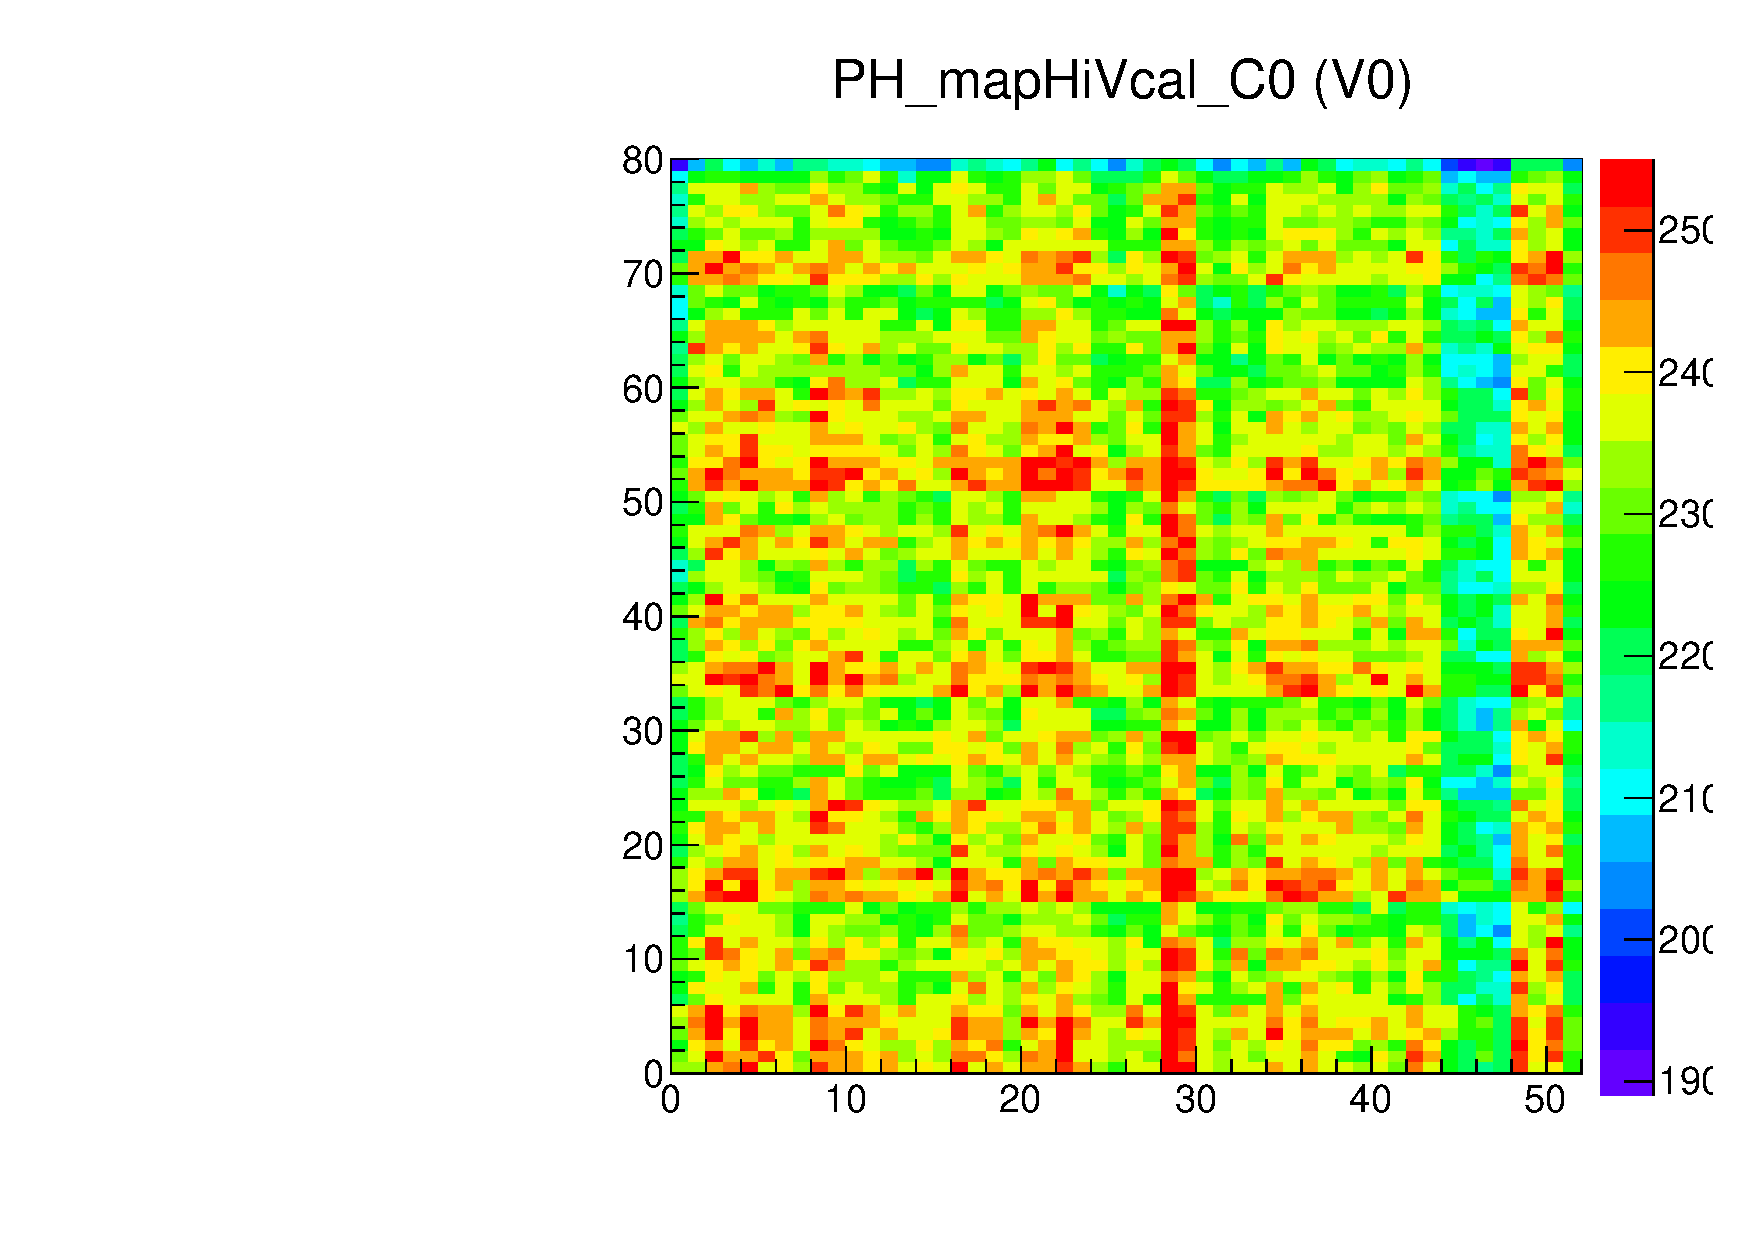
\includegraphics[width=1.0\textwidth]{figures/phopt_PH_mapHiVcal.pdf}
  \caption{\roc map of pulse heights with \vcal set to target ADC saturation point.}
  \label{fig:phopt_PH_mapHiVcal}
\end{minipage}
\hspace{0.3cm}
\begin{minipage}{0.45\textwidth}
  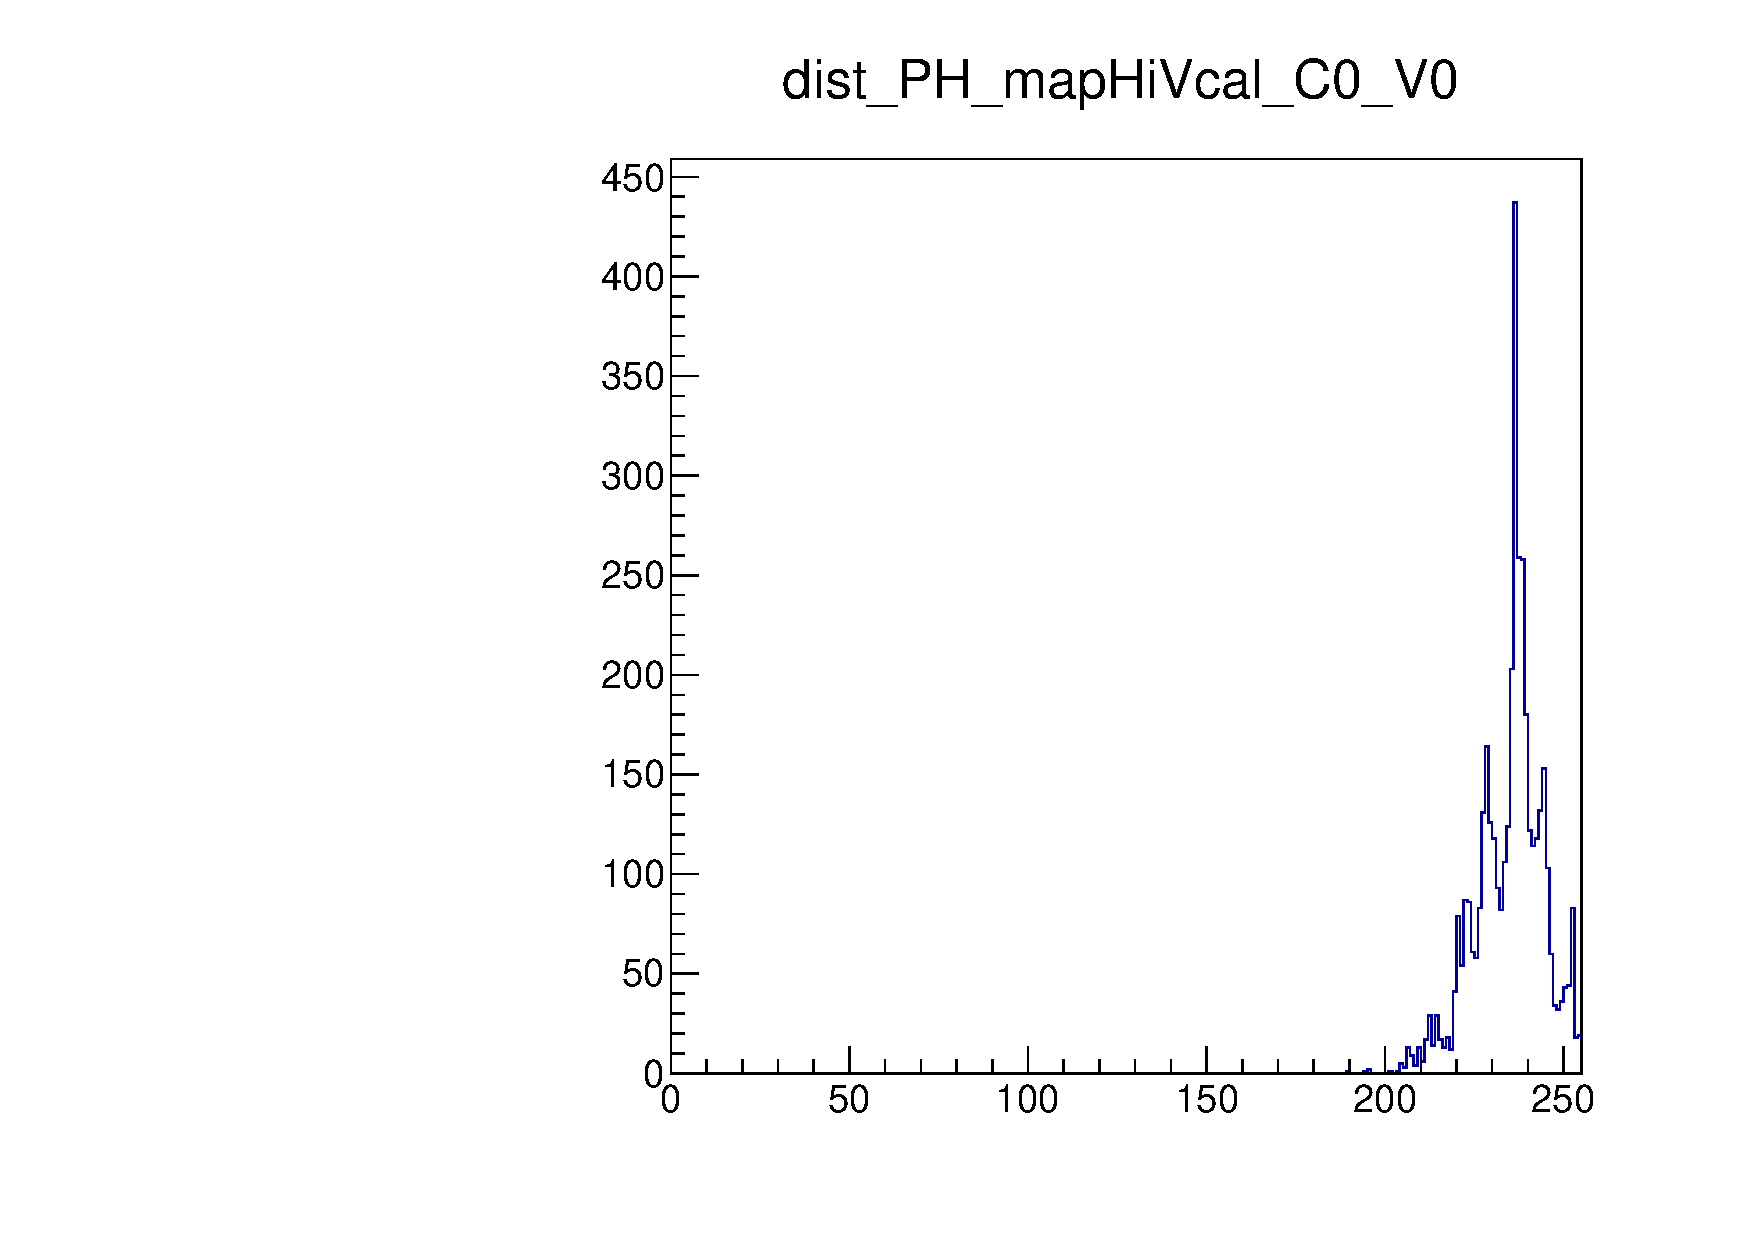
\includegraphics[width=1.0\textwidth]{figures/phopt_dist_PH_mapHiVcal.pdf}
  \caption{1D distribution of Figure~\ref{fig:phopt_PH_mapHiVcal}.}
  \label{fig:phopt_dist_PH_mapHiVcal}
\end{minipage}
\end{figure}

